% Options for packages loaded elsewhere
\PassOptionsToPackage{unicode}{hyperref}
\PassOptionsToPackage{hyphens}{url}
%
\documentclass[
]{article}
\usepackage{lmodern}
\usepackage{amssymb,amsmath}
\usepackage{ifxetex,ifluatex}
\ifnum 0\ifxetex 1\fi\ifluatex 1\fi=0 % if pdftex
  \usepackage[T1]{fontenc}
  \usepackage[utf8]{inputenc}
  \usepackage{textcomp} % provide euro and other symbols
\else % if luatex or xetex
  \usepackage{unicode-math}
  \defaultfontfeatures{Scale=MatchLowercase}
  \defaultfontfeatures[\rmfamily]{Ligatures=TeX,Scale=1}
\fi
% Use upquote if available, for straight quotes in verbatim environments
\IfFileExists{upquote.sty}{\usepackage{upquote}}{}
\IfFileExists{microtype.sty}{% use microtype if available
  \usepackage[]{microtype}
  \UseMicrotypeSet[protrusion]{basicmath} % disable protrusion for tt fonts
}{}
\makeatletter
\@ifundefined{KOMAClassName}{% if non-KOMA class
  \IfFileExists{parskip.sty}{%
    \usepackage{parskip}
  }{% else
    \setlength{\parindent}{0pt}
    \setlength{\parskip}{6pt plus 2pt minus 1pt}}
}{% if KOMA class
  \KOMAoptions{parskip=half}}
\makeatother
\usepackage{xcolor}
\IfFileExists{xurl.sty}{\usepackage{xurl}}{} % add URL line breaks if available
\IfFileExists{bookmark.sty}{\usepackage{bookmark}}{\usepackage{hyperref}}
\hypersetup{
  pdftitle={Project on CPU, GPU, and TPU},
  pdfauthor={Lixian Chen, Zhanhao Zhang, Jingbin Cao},
  hidelinks,
  pdfcreator={LaTeX via pandoc}}
\urlstyle{same} % disable monospaced font for URLs
\usepackage[margin=1in]{geometry}
\usepackage{color}
\usepackage{fancyvrb}
\newcommand{\VerbBar}{|}
\newcommand{\VERB}{\Verb[commandchars=\\\{\}]}
\DefineVerbatimEnvironment{Highlighting}{Verbatim}{commandchars=\\\{\}}
% Add ',fontsize=\small' for more characters per line
\usepackage{framed}
\definecolor{shadecolor}{RGB}{248,248,248}
\newenvironment{Shaded}{\begin{snugshade}}{\end{snugshade}}
\newcommand{\AlertTok}[1]{\textcolor[rgb]{0.94,0.16,0.16}{#1}}
\newcommand{\AnnotationTok}[1]{\textcolor[rgb]{0.56,0.35,0.01}{\textbf{\textit{#1}}}}
\newcommand{\AttributeTok}[1]{\textcolor[rgb]{0.77,0.63,0.00}{#1}}
\newcommand{\BaseNTok}[1]{\textcolor[rgb]{0.00,0.00,0.81}{#1}}
\newcommand{\BuiltInTok}[1]{#1}
\newcommand{\CharTok}[1]{\textcolor[rgb]{0.31,0.60,0.02}{#1}}
\newcommand{\CommentTok}[1]{\textcolor[rgb]{0.56,0.35,0.01}{\textit{#1}}}
\newcommand{\CommentVarTok}[1]{\textcolor[rgb]{0.56,0.35,0.01}{\textbf{\textit{#1}}}}
\newcommand{\ConstantTok}[1]{\textcolor[rgb]{0.00,0.00,0.00}{#1}}
\newcommand{\ControlFlowTok}[1]{\textcolor[rgb]{0.13,0.29,0.53}{\textbf{#1}}}
\newcommand{\DataTypeTok}[1]{\textcolor[rgb]{0.13,0.29,0.53}{#1}}
\newcommand{\DecValTok}[1]{\textcolor[rgb]{0.00,0.00,0.81}{#1}}
\newcommand{\DocumentationTok}[1]{\textcolor[rgb]{0.56,0.35,0.01}{\textbf{\textit{#1}}}}
\newcommand{\ErrorTok}[1]{\textcolor[rgb]{0.64,0.00,0.00}{\textbf{#1}}}
\newcommand{\ExtensionTok}[1]{#1}
\newcommand{\FloatTok}[1]{\textcolor[rgb]{0.00,0.00,0.81}{#1}}
\newcommand{\FunctionTok}[1]{\textcolor[rgb]{0.00,0.00,0.00}{#1}}
\newcommand{\ImportTok}[1]{#1}
\newcommand{\InformationTok}[1]{\textcolor[rgb]{0.56,0.35,0.01}{\textbf{\textit{#1}}}}
\newcommand{\KeywordTok}[1]{\textcolor[rgb]{0.13,0.29,0.53}{\textbf{#1}}}
\newcommand{\NormalTok}[1]{#1}
\newcommand{\OperatorTok}[1]{\textcolor[rgb]{0.81,0.36,0.00}{\textbf{#1}}}
\newcommand{\OtherTok}[1]{\textcolor[rgb]{0.56,0.35,0.01}{#1}}
\newcommand{\PreprocessorTok}[1]{\textcolor[rgb]{0.56,0.35,0.01}{\textit{#1}}}
\newcommand{\RegionMarkerTok}[1]{#1}
\newcommand{\SpecialCharTok}[1]{\textcolor[rgb]{0.00,0.00,0.00}{#1}}
\newcommand{\SpecialStringTok}[1]{\textcolor[rgb]{0.31,0.60,0.02}{#1}}
\newcommand{\StringTok}[1]{\textcolor[rgb]{0.31,0.60,0.02}{#1}}
\newcommand{\VariableTok}[1]{\textcolor[rgb]{0.00,0.00,0.00}{#1}}
\newcommand{\VerbatimStringTok}[1]{\textcolor[rgb]{0.31,0.60,0.02}{#1}}
\newcommand{\WarningTok}[1]{\textcolor[rgb]{0.56,0.35,0.01}{\textbf{\textit{#1}}}}
\usepackage{graphicx}
\makeatletter
\def\maxwidth{\ifdim\Gin@nat@width>\linewidth\linewidth\else\Gin@nat@width\fi}
\def\maxheight{\ifdim\Gin@nat@height>\textheight\textheight\else\Gin@nat@height\fi}
\makeatother
% Scale images if necessary, so that they will not overflow the page
% margins by default, and it is still possible to overwrite the defaults
% using explicit options in \includegraphics[width, height, ...]{}
\setkeys{Gin}{width=\maxwidth,height=\maxheight,keepaspectratio}
% Set default figure placement to htbp
\makeatletter
\def\fps@figure{htbp}
\makeatother
\setlength{\emergencystretch}{3em} % prevent overfull lines
\providecommand{\tightlist}{%
  \setlength{\itemsep}{0pt}\setlength{\parskip}{0pt}}
\setcounter{secnumdepth}{-\maxdimen} % remove section numbering
\usepackage{graphicx}

\title{Project on CPU, GPU, and TPU}
\author{Lixian Chen, Zhanhao Zhang, Jingbin Cao}
\date{4/14/2021}

\begin{document}
\maketitle

\hypertarget{preparing-required-packages}{%
\section{Preparing Required
Packages}\label{preparing-required-packages}}

\hypertarget{read-data}{%
\section{Read Data}\label{read-data}}

\begin{Shaded}
\begin{Highlighting}[]
\NormalTok{data \textless{}{-}}\StringTok{ }\KeywordTok{read.csv}\NormalTok{(}\StringTok{"../data/Runtime.csv"}\NormalTok{)}
\KeywordTok{head}\NormalTok{(data)}
\end{Highlighting}
\end{Shaded}

\begin{verbatim}
##       Runtime Processor MatrixSize MatrixOperation Trial
## 1 0.003411770       CPU         10        Addition     1
## 2 0.006412983       CPU         10        Addition     2
## 3 0.003450394       CPU         10        Addition     3
## 4 0.003098965       CPU         10        Addition     4
## 5 0.002490997       CPU         10        Addition     5
## 6 0.002594948       CPU         20        Addition     1
\end{verbatim}

We tested three types of processors CPU, GPU, and TPU for three kinds of
matrix operation, addition, multiplication, and inversion, with the
matrix from size 10 to size 2160. We repeat each test for five times.\\
\textbf{We measured log10(run-time) for each trial, and we use that as
the evaluation of the performances.}

\hypertarget{simple-plots}{%
\section{Simple Plots}\label{simple-plots}}

Here is the general visualization for the performances of each processor
under three matrix operations:

\begin{Shaded}
\begin{Highlighting}[]
\KeywordTok{jpeg}\NormalTok{(}\DataTypeTok{filename =} \StringTok{"../figs/overview.jpeg"}\NormalTok{, }\DataTypeTok{width =} \DecValTok{1000}\NormalTok{, }\DataTypeTok{height =} \DecValTok{800}\NormalTok{,}\DataTypeTok{quality =} \DecValTok{10000}\NormalTok{)}
\KeywordTok{ggplot}\NormalTok{(}\DataTypeTok{data =}\NormalTok{ data, }\KeywordTok{aes}\NormalTok{(}\DataTypeTok{x =}\NormalTok{ Processor, }\DataTypeTok{y =} \KeywordTok{log10}\NormalTok{(Runtime))) }\OperatorTok{+}
\KeywordTok{geom\_boxplot}\NormalTok{(}\KeywordTok{aes}\NormalTok{(}\DataTypeTok{fill =}\NormalTok{ MatrixOperation))}
\ControlFlowTok{while}\NormalTok{ (}\OperatorTok{!}\KeywordTok{is.null}\NormalTok{(}\KeywordTok{dev.list}\NormalTok{()))  }\KeywordTok{dev.off}\NormalTok{()}
\end{Highlighting}
\end{Shaded}

\begin{center}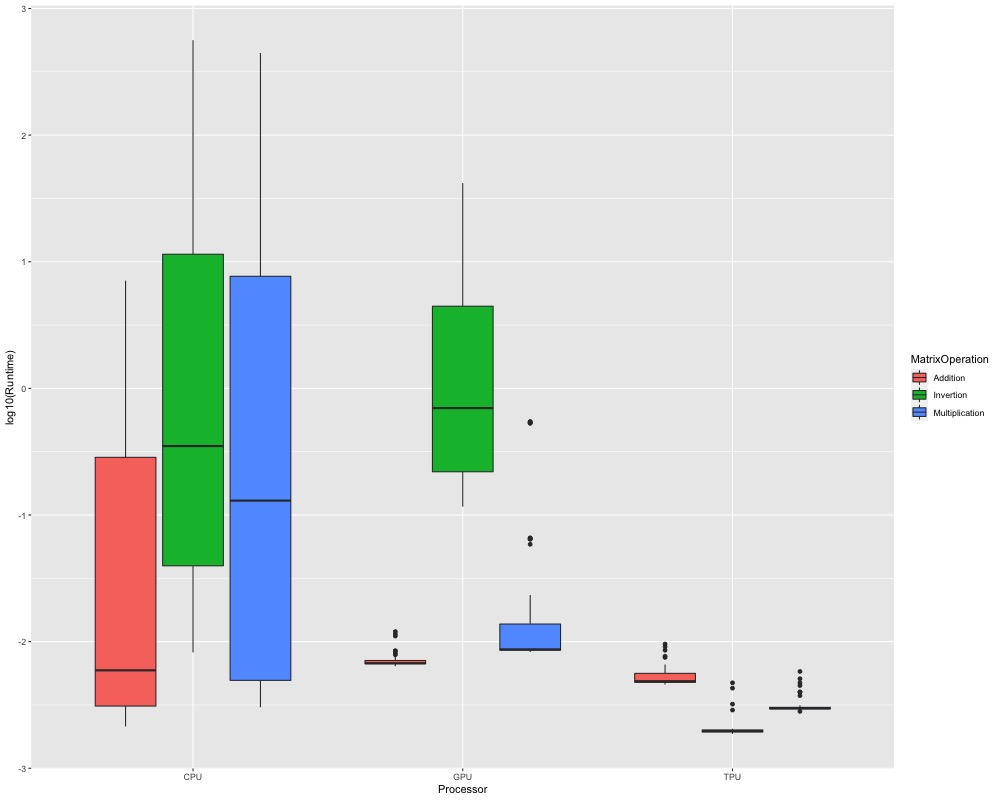
\includegraphics[width=0.9\linewidth]{../figs/overview} \end{center}

\hypertarget{jingbin-cao-part-i}{%
\section{Jingbin Cao Part I}\label{jingbin-cao-part-i}}

One Way Anova for different matrix sized for each pair of processor and
matrix operation: \(\mu_0 = Matrix_{Size}=320\)
\(\mu_1 = Matrix_{Size}=640\) \(\mu_2 = Matrix_{Size}=1280\)
\(\mu_3 = Matrix_{Size}=2160\)

\hypertarget{getting-data}{%
\subsection{Getting Data}\label{getting-data}}

\begin{Shaded}
\begin{Highlighting}[]
\NormalTok{cpu\_add \textless{}{-}}\StringTok{ }\NormalTok{data[data}\OperatorTok{$}\NormalTok{Processor }\OperatorTok{==}\StringTok{ "CPU"} \OperatorTok{\&}\StringTok{ }\NormalTok{data}\OperatorTok{$}\NormalTok{MatrixOperation}\OperatorTok{==}\StringTok{"Addition"} \OperatorTok{\&}\StringTok{ }\NormalTok{data}\OperatorTok{$}\NormalTok{MatrixSize }\OperatorTok{\textgreater{}=}\StringTok{ }\DecValTok{320}\NormalTok{,]}
\NormalTok{cpu\_mult \textless{}{-}}\StringTok{ }\NormalTok{data[data}\OperatorTok{$}\NormalTok{Processor }\OperatorTok{==}\StringTok{ "CPU"} \OperatorTok{\&}\StringTok{ }\NormalTok{data}\OperatorTok{$}\NormalTok{MatrixOperation}\OperatorTok{==}\StringTok{"Multiplication"} \OperatorTok{\&}\StringTok{ }\NormalTok{data}\OperatorTok{$}\NormalTok{MatrixSize }\OperatorTok{\textgreater{}=}\StringTok{ }\DecValTok{320}\NormalTok{,]}
\NormalTok{cpu\_inv \textless{}{-}}\StringTok{ }\NormalTok{data[data}\OperatorTok{$}\NormalTok{Processor }\OperatorTok{==}\StringTok{ "CPU"} \OperatorTok{\&}\StringTok{ }\NormalTok{data}\OperatorTok{$}\NormalTok{MatrixOperation}\OperatorTok{==}\StringTok{"Invertion"} \OperatorTok{\&}\StringTok{ }\NormalTok{data}\OperatorTok{$}\NormalTok{MatrixSize }\OperatorTok{\textgreater{}=}\StringTok{ }\DecValTok{320}\NormalTok{,]}
\NormalTok{gpu\_add \textless{}{-}}\StringTok{ }\NormalTok{data[data}\OperatorTok{$}\NormalTok{Processor }\OperatorTok{==}\StringTok{ "GPU"} \OperatorTok{\&}\StringTok{ }\NormalTok{data}\OperatorTok{$}\NormalTok{MatrixOperation}\OperatorTok{==}\StringTok{"Addition"} \OperatorTok{\&}\StringTok{ }\NormalTok{data}\OperatorTok{$}\NormalTok{MatrixSize }\OperatorTok{\textgreater{}=}\StringTok{ }\DecValTok{320}\NormalTok{,]}
\NormalTok{gpu\_mult \textless{}{-}}\StringTok{ }\NormalTok{data[data}\OperatorTok{$}\NormalTok{Processor }\OperatorTok{==}\StringTok{ "GPU"} \OperatorTok{\&}\StringTok{ }\NormalTok{data}\OperatorTok{$}\NormalTok{MatrixOperation}\OperatorTok{==}\StringTok{"Multiplication"} \OperatorTok{\&}\StringTok{ }\NormalTok{data}\OperatorTok{$}\NormalTok{MatrixSize }\OperatorTok{\textgreater{}=}\StringTok{ }\DecValTok{320}\NormalTok{,]}
\NormalTok{gpu\_inv \textless{}{-}}\StringTok{ }\NormalTok{data[data}\OperatorTok{$}\NormalTok{Processor }\OperatorTok{==}\StringTok{ "GPU"} \OperatorTok{\&}\StringTok{ }\NormalTok{data}\OperatorTok{$}\NormalTok{MatrixOperation}\OperatorTok{==}\StringTok{"Invertion"} \OperatorTok{\&}\StringTok{ }\NormalTok{data}\OperatorTok{$}\NormalTok{MatrixSize }\OperatorTok{\textgreater{}=}\StringTok{ }\DecValTok{320}\NormalTok{,]}
\NormalTok{tpu\_add \textless{}{-}}\StringTok{ }\NormalTok{data[data}\OperatorTok{$}\NormalTok{Processor }\OperatorTok{==}\StringTok{ "TPU"} \OperatorTok{\&}\StringTok{ }\NormalTok{data}\OperatorTok{$}\NormalTok{MatrixOperation}\OperatorTok{==}\StringTok{"Addition"} \OperatorTok{\&}\StringTok{ }\NormalTok{data}\OperatorTok{$}\NormalTok{MatrixSize }\OperatorTok{\textgreater{}=}\StringTok{ }\DecValTok{320}\NormalTok{,]}
\NormalTok{tpu\_mult \textless{}{-}}\StringTok{ }\NormalTok{data[data}\OperatorTok{$}\NormalTok{Processor }\OperatorTok{==}\StringTok{ "TPU"} \OperatorTok{\&}\StringTok{ }\NormalTok{data}\OperatorTok{$}\NormalTok{MatrixOperation}\OperatorTok{==}\StringTok{"Multiplication"} \OperatorTok{\&}\StringTok{ }\NormalTok{data}\OperatorTok{$}\NormalTok{MatrixSize }\OperatorTok{\textgreater{}=}\StringTok{ }\DecValTok{320}\NormalTok{,]}
\NormalTok{tpu\_inv \textless{}{-}}\StringTok{ }\NormalTok{data[data}\OperatorTok{$}\NormalTok{Processor }\OperatorTok{==}\StringTok{ "TPU"} \OperatorTok{\&}\StringTok{ }\NormalTok{data}\OperatorTok{$}\NormalTok{MatrixOperation}\OperatorTok{==}\StringTok{"Invertion"} \OperatorTok{\&}\StringTok{ }\NormalTok{data}\OperatorTok{$}\NormalTok{MatrixSize }\OperatorTok{\textgreater{}=}\StringTok{ }\DecValTok{320}\NormalTok{,]}
\end{Highlighting}
\end{Shaded}

\hypertarget{anovas}{%
\subsection{Anovas}\label{anovas}}

\begin{Shaded}
\begin{Highlighting}[]
\KeywordTok{summary}\NormalTok{(}\KeywordTok{aov}\NormalTok{(Runtime }\OperatorTok{\textasciitilde{}}\StringTok{ }\NormalTok{MatrixSize, }\DataTypeTok{data=}\NormalTok{cpu\_add))}
\end{Highlighting}
\end{Shaded}

\begin{verbatim}
##             Df Sum Sq Mean Sq F value   Pr(>F)    
## MatrixSize   1 152.37  152.37   338.2 4.08e-13 ***
## Residuals   18   8.11    0.45                     
## ---
## Signif. codes:  0 '***' 0.001 '**' 0.01 '*' 0.05 '.' 0.1 ' ' 1
\end{verbatim}

\begin{Shaded}
\begin{Highlighting}[]
\KeywordTok{summary}\NormalTok{(}\KeywordTok{aov}\NormalTok{(Runtime }\OperatorTok{\textasciitilde{}}\StringTok{ }\NormalTok{MatrixSize, }\DataTypeTok{data=}\NormalTok{cpu\_mult))}
\end{Highlighting}
\end{Shaded}

\begin{verbatim}
##             Df Sum Sq Mean Sq F value  Pr(>F)    
## MatrixSize   1 619133  619133   187.8 5.8e-11 ***
## Residuals   18  59356    3298                    
## ---
## Signif. codes:  0 '***' 0.001 '**' 0.01 '*' 0.05 '.' 0.1 ' ' 1
\end{verbatim}

\begin{Shaded}
\begin{Highlighting}[]
\KeywordTok{summary}\NormalTok{(}\KeywordTok{aov}\NormalTok{(Runtime }\OperatorTok{\textasciitilde{}}\StringTok{ }\NormalTok{MatrixSize, }\DataTypeTok{data=}\NormalTok{cpu\_inv))}
\end{Highlighting}
\end{Shaded}

\begin{verbatim}
##             Df Sum Sq Mean Sq F value   Pr(>F)    
## MatrixSize   1 984766  984766   203.7 2.95e-11 ***
## Residuals   18  87022    4835                     
## ---
## Signif. codes:  0 '***' 0.001 '**' 0.01 '*' 0.05 '.' 0.1 ' ' 1
\end{verbatim}

\begin{Shaded}
\begin{Highlighting}[]
\KeywordTok{summary}\NormalTok{(}\KeywordTok{aov}\NormalTok{(Runtime }\OperatorTok{\textasciitilde{}}\StringTok{ }\NormalTok{MatrixSize, }\DataTypeTok{data=}\NormalTok{gpu\_add))}
\end{Highlighting}
\end{Shaded}

\begin{verbatim}
##             Df    Sum Sq   Mean Sq F value Pr(>F)
## MatrixSize   1 1.200e-07 1.250e-07   0.038  0.847
## Residuals   18 5.845e-05 3.247e-06
\end{verbatim}

\begin{Shaded}
\begin{Highlighting}[]
\KeywordTok{summary}\NormalTok{(}\KeywordTok{aov}\NormalTok{(Runtime }\OperatorTok{\textasciitilde{}}\StringTok{ }\NormalTok{MatrixSize, }\DataTypeTok{data=}\NormalTok{gpu\_mult))}
\end{Highlighting}
\end{Shaded}

\begin{verbatim}
##             Df Sum Sq Mean Sq F value Pr(>F)
## MatrixSize   1 0.0003 0.00025   0.005  0.947
## Residuals   18 0.9873 0.05485
\end{verbatim}

\begin{Shaded}
\begin{Highlighting}[]
\KeywordTok{summary}\NormalTok{(}\KeywordTok{aov}\NormalTok{(Runtime }\OperatorTok{\textasciitilde{}}\StringTok{ }\NormalTok{MatrixSize, }\DataTypeTok{data=}\NormalTok{gpu\_inv))}
\end{Highlighting}
\end{Shaded}

\begin{verbatim}
##             Df Sum Sq Mean Sq F value   Pr(>F)    
## MatrixSize   1   4896    4896   476.7 2.11e-14 ***
## Residuals   18    185      10                     
## ---
## Signif. codes:  0 '***' 0.001 '**' 0.01 '*' 0.05 '.' 0.1 ' ' 1
\end{verbatim}

\begin{Shaded}
\begin{Highlighting}[]
\KeywordTok{summary}\NormalTok{(}\KeywordTok{aov}\NormalTok{(Runtime }\OperatorTok{\textasciitilde{}}\StringTok{ }\NormalTok{MatrixSize, }\DataTypeTok{data=}\NormalTok{tpu\_add))}
\end{Highlighting}
\end{Shaded}

\begin{verbatim}
##             Df    Sum Sq   Mean Sq F value Pr(>F)
## MatrixSize   1 1.000e-08 9.800e-09   0.006   0.94
## Residuals   18 2.993e-05 1.663e-06
\end{verbatim}

\begin{Shaded}
\begin{Highlighting}[]
\KeywordTok{summary}\NormalTok{(}\KeywordTok{aov}\NormalTok{(Runtime }\OperatorTok{\textasciitilde{}}\StringTok{ }\NormalTok{MatrixSize, }\DataTypeTok{data=}\NormalTok{tpu\_mult))}
\end{Highlighting}
\end{Shaded}

\begin{verbatim}
##             Df    Sum Sq   Mean Sq F value Pr(>F)
## MatrixSize   1 1.200e-08 1.210e-08   0.028  0.869
## Residuals   18 7.745e-06 4.303e-07
\end{verbatim}

\begin{Shaded}
\begin{Highlighting}[]
\KeywordTok{summary}\NormalTok{(}\KeywordTok{aov}\NormalTok{(Runtime }\OperatorTok{\textasciitilde{}}\StringTok{ }\NormalTok{MatrixSize, }\DataTypeTok{data=}\NormalTok{tpu\_inv))}
\end{Highlighting}
\end{Shaded}

\begin{verbatim}
##             Df    Sum Sq   Mean Sq F value Pr(>F)
## MatrixSize   1 3.300e-07 3.301e-07    1.13  0.302
## Residuals   18 5.258e-06 2.921e-07
\end{verbatim}

\hypertarget{zhanhao-zhang-part-i}{%
\section{Zhanhao Zhang Part I}\label{zhanhao-zhang-part-i}}

\hypertarget{pros-cons-of-each-processor}{%
\subsection{Pros \& Cons of Each
Processor}\label{pros-cons-of-each-processor}}

When matrix size is the same, is there any processor or operation
effects? Or is there any interactive effect?

\begin{Shaded}
\begin{Highlighting}[]
\NormalTok{df\_cpu \textless{}{-}}\StringTok{ }\NormalTok{data[data}\OperatorTok{$}\NormalTok{Processor }\OperatorTok{==}\StringTok{ "CPU"}\NormalTok{,]}
\KeywordTok{lm}\NormalTok{(Runtime }\OperatorTok{\textasciitilde{}}\StringTok{ }\NormalTok{MatrixSize }\OperatorTok{+}\StringTok{ }\KeywordTok{as.factor}\NormalTok{(MatrixOperation), }\DataTypeTok{data =}\NormalTok{ df\_cpu) }\OperatorTok{\%\textgreater{}\%}
\StringTok{  }\KeywordTok{summary}\NormalTok{()}
\end{Highlighting}
\end{Shaded}

\begin{verbatim}
## 
## Call:
## lm(formula = Runtime ~ MatrixSize + as.factor(MatrixOperation), 
##     data = df_cpu)
## 
## Residuals:
##      Min       1Q   Median       3Q      Max 
## -234.810  -41.042   -6.483   48.307  248.752 
## 
## Coefficients:
##                                            Estimate Std. Error t value Pr(>|t|)
## (Intercept)                              -67.641331  13.699933  -4.937 2.37e-06
## MatrixSize                                 0.120877   0.009097  13.287  < 2e-16
## as.factor(MatrixOperation)Invertion       71.726373  17.944905   3.997 0.000107
## as.factor(MatrixOperation)Multiplication  55.821041  17.944905   3.111 0.002291
##                                             
## (Intercept)                              ***
## MatrixSize                               ***
## as.factor(MatrixOperation)Invertion      ***
## as.factor(MatrixOperation)Multiplication ** 
## ---
## Signif. codes:  0 '***' 0.001 '**' 0.01 '*' 0.05 '.' 0.1 ' ' 1
## 
## Residual standard error: 85.12 on 131 degrees of freedom
## Multiple R-squared:  0.5971, Adjusted R-squared:  0.5879 
## F-statistic: 64.73 on 3 and 131 DF,  p-value: < 2.2e-16
\end{verbatim}

\begin{Shaded}
\begin{Highlighting}[]
\NormalTok{df\_tpu \textless{}{-}}\StringTok{ }\NormalTok{data[data}\OperatorTok{$}\NormalTok{Processor }\OperatorTok{==}\StringTok{ "TPU"}\NormalTok{,]}
\KeywordTok{lm}\NormalTok{(Runtime }\OperatorTok{\textasciitilde{}}\StringTok{ }\NormalTok{MatrixSize }\OperatorTok{+}\StringTok{ }\KeywordTok{as.factor}\NormalTok{(MatrixOperation), }\DataTypeTok{data =}\NormalTok{ df\_tpu) }\OperatorTok{\%\textgreater{}\%}
\StringTok{  }\KeywordTok{summary}\NormalTok{()}
\end{Highlighting}
\end{Shaded}

\begin{verbatim}
## 
## Call:
## lm(formula = Runtime ~ MatrixSize + as.factor(MatrixOperation), 
##     data = df_tpu)
## 
## Residuals:
##        Min         1Q     Median         3Q        Max 
## -0.0008794 -0.0003316 -0.0002244 -0.0000993  0.0041166 
## 
## Coefficients:
##                                            Estimate Std. Error t value Pr(>|t|)
## (Intercept)                               5.460e-03  1.389e-04  39.296   <2e-16
## MatrixSize                               -2.635e-08  9.226e-08  -0.286    0.776
## as.factor(MatrixOperation)Invertion      -3.320e-03  1.820e-04 -18.243   <2e-16
## as.factor(MatrixOperation)Multiplication -2.238e-03  1.820e-04 -12.296   <2e-16
##                                             
## (Intercept)                              ***
## MatrixSize                                  
## as.factor(MatrixOperation)Invertion      ***
## as.factor(MatrixOperation)Multiplication ***
## ---
## Signif. codes:  0 '***' 0.001 '**' 0.01 '*' 0.05 '.' 0.1 ' ' 1
## 
## Residual standard error: 0.0008633 on 131 degrees of freedom
## Multiple R-squared:  0.7256, Adjusted R-squared:  0.7193 
## F-statistic: 115.4 on 3 and 131 DF,  p-value: < 2.2e-16
\end{verbatim}

\begin{Shaded}
\begin{Highlighting}[]
\NormalTok{df\_gpu \textless{}{-}}\StringTok{ }\NormalTok{data[data}\OperatorTok{$}\NormalTok{Processor }\OperatorTok{==}\StringTok{ "GPU"}\NormalTok{,]}
\KeywordTok{lm}\NormalTok{(Runtime }\OperatorTok{\textasciitilde{}}\StringTok{ }\NormalTok{MatrixSize }\OperatorTok{+}\StringTok{ }\KeywordTok{as.factor}\NormalTok{(MatrixOperation), }\DataTypeTok{data =}\NormalTok{ df\_gpu) }\OperatorTok{\%\textgreater{}\%}
\StringTok{  }\KeywordTok{summary}\NormalTok{()}
\end{Highlighting}
\end{Shaded}

\begin{verbatim}
## 
## Call:
## lm(formula = Runtime ~ MatrixSize + as.factor(MatrixOperation), 
##     data = df_gpu)
## 
## Residuals:
##      Min       1Q   Median       3Q      Max 
## -10.4178  -3.7532   0.9807   2.6766  24.7084 
## 
## Coefficients:
##                                            Estimate Std. Error t value Pr(>|t|)
## (Intercept)                              -2.9430365  1.0021808  -2.937  0.00392
## MatrixSize                                0.0051962  0.0006655   7.808 1.64e-12
## as.factor(MatrixOperation)Invertion       6.7906886  1.3127100   5.173 8.42e-07
## as.factor(MatrixOperation)Multiplication  0.0669200  1.3127100   0.051  0.95942
##                                             
## (Intercept)                              ** 
## MatrixSize                               ***
## as.factor(MatrixOperation)Invertion      ***
## as.factor(MatrixOperation)Multiplication    
## ---
## Signif. codes:  0 '***' 0.001 '**' 0.01 '*' 0.05 '.' 0.1 ' ' 1
## 
## Residual standard error: 6.227 on 131 degrees of freedom
## Multiple R-squared:  0.4237, Adjusted R-squared:  0.4105 
## F-statistic:  32.1 on 3 and 131 DF,  p-value: 1.273e-15
\end{verbatim}

\hypertarget{lixian-chen-part-i}{%
\section{Lixian Chen Part I}\label{lixian-chen-part-i}}

When the processor is the same, is there any operation and matrix size
effect? We want to answer the following question: in each scenario,
which processor should we use?

\hypertarget{getting-data-ready}{%
\subsection{Getting Data Ready}\label{getting-data-ready}}

\begin{Shaded}
\begin{Highlighting}[]
\CommentTok{\# Read Data}
\NormalTok{df \textless{}{-}}\StringTok{ }\KeywordTok{fread}\NormalTok{(}\StringTok{"../data/Runtime.csv"}\NormalTok{, }\DataTypeTok{header=}\OtherTok{TRUE}\NormalTok{)}
\KeywordTok{attach}\NormalTok{(df)}

\NormalTok{MatrixOperation\textless{}{-}}\KeywordTok{factor}\NormalTok{(MatrixOperation)}
\NormalTok{Processor\textless{}{-}}\KeywordTok{factor}\NormalTok{(Processor)}



\NormalTok{CPUdata \textless{}{-}}\StringTok{ }\NormalTok{df }\OperatorTok{\%\textgreater{}\%}\StringTok{ }\KeywordTok{filter}\NormalTok{(Processor}\OperatorTok{==}\StringTok{"CPU"}\NormalTok{)}
\NormalTok{GPUdata \textless{}{-}}\StringTok{ }\NormalTok{df }\OperatorTok{\%\textgreater{}\%}\StringTok{ }\KeywordTok{filter}\NormalTok{(Processor}\OperatorTok{==}\StringTok{"GPU"}\NormalTok{)}
\NormalTok{TPUdata \textless{}{-}}\StringTok{ }\NormalTok{df }\OperatorTok{\%\textgreater{}\%}\StringTok{ }\KeywordTok{filter}\NormalTok{(Processor}\OperatorTok{==}\StringTok{"TPU"}\NormalTok{)}



\KeywordTok{describeBy}\NormalTok{(df}\OperatorTok{$}\NormalTok{Runtime,}\DataTypeTok{group =}\NormalTok{ df}\OperatorTok{$}\NormalTok{MatrixSize, }\DataTypeTok{mat =} \OtherTok{TRUE}\NormalTok{) }\OperatorTok{\%\textgreater{}\%}\StringTok{  }\CommentTok{\#create dataframe}
\StringTok{  }\KeywordTok{select}\NormalTok{(}\DataTypeTok{MatrixSize=}\NormalTok{group1, }\DataTypeTok{N=}\NormalTok{n, }\DataTypeTok{Mean=}\NormalTok{mean, }\DataTypeTok{SD=}\NormalTok{sd, }\DataTypeTok{Median=}\NormalTok{median, }\DataTypeTok{Min=}\NormalTok{min, }\DataTypeTok{Max=}\NormalTok{max, }
         \DataTypeTok{Skew=}\NormalTok{skew, }\DataTypeTok{Kurtosis=}\NormalTok{kurtosis, }\DataTypeTok{SEM=}\NormalTok{se)}
\end{Highlighting}
\end{Shaded}

\begin{verbatim}
##     MatrixSize  N         Mean           SD      Median         Min         Max
## X11         10 45   0.02117285   0.04190229 0.005617142 0.001893044   0.1475253
## X12         20 45   0.02285517   0.04503445 0.004884481 0.001916409   0.1613362
## X13         40 45   0.03386522   0.07211264 0.005309582 0.001902819   0.2506576
## X14         80 45   0.06023479   0.12131721 0.006777525 0.001910210   0.4039948
## X15        160 45   0.13455488   0.22988237 0.006753206 0.001870394   0.7055206
## X16        320 45   0.54802946   0.77266887 0.008684158 0.001933098   1.8301501
## X17        640 45   2.65963363   4.07807665 0.064900875 0.001965523  11.5108950
## X18       1280 45  16.76243327  28.75264487 0.538181782 0.001962900  80.1931298
## X19       2560 45 117.16431474 210.69591026 0.008469582 0.001975775 562.2822752
##          Skew    Kurtosis          SEM
## X11 2.2815817  3.52258988  0.006246425
## X12 2.2598210  3.47569251  0.006713340
## X13 2.3149204  3.63635579  0.010749918
## X14 2.1514343  3.03908564  0.018084903
## X15 1.6153802  1.18296414  0.034268841
## X16 0.7633051 -1.35170085  0.115182675
## X17 1.1600905 -0.21560402  0.607923773
## X18 1.3579285  0.07252682  4.286191230
## X19 1.3393614 -0.10016629 31.408691862
\end{verbatim}

\begin{Shaded}
\begin{Highlighting}[]
\CommentTok{\#boxplot(Runtime\textasciitilde{}Processor*MatrixOperation)}
\CommentTok{\#tapply(Runtime,list(Processor, MatrixOperation),mean)}
\CommentTok{\#tapply(Runtime,MatrixOperation,mean)}

\KeywordTok{group\_by}\NormalTok{(df, Processor) }\OperatorTok{\%\textgreater{}\%}
\StringTok{  }\KeywordTok{summarise}\NormalTok{(}
    \DataTypeTok{count =} \KeywordTok{n}\NormalTok{(),}
    \DataTypeTok{mean =} \KeywordTok{mean}\NormalTok{(Runtime, }\DataTypeTok{na.rm =} \OtherTok{TRUE}\NormalTok{),}
    \DataTypeTok{sd =} \KeywordTok{sd}\NormalTok{(Runtime, }\DataTypeTok{na.rm =} \OtherTok{TRUE}\NormalTok{)}
\NormalTok{  )}
\end{Highlighting}
\end{Shaded}

\begin{verbatim}
## # A tibble: 3 x 4
##   Processor count     mean        sd
##   <chr>     <int>    <dbl>     <dbl>
## 1 CPU         135 43.5     133.     
## 2 GPU         135  2.29      8.11   
## 3 TPU         135  0.00359   0.00163
\end{verbatim}

\begin{Shaded}
\begin{Highlighting}[]
\KeywordTok{group\_by}\NormalTok{(df, MatrixOperation) }\OperatorTok{\%\textgreater{}\%}
\StringTok{  }\KeywordTok{summarise}\NormalTok{(}
    \DataTypeTok{count =} \KeywordTok{n}\NormalTok{(),}
    \DataTypeTok{mean =} \KeywordTok{mean}\NormalTok{(Runtime, }\DataTypeTok{na.rm =} \OtherTok{TRUE}\NormalTok{),}
    \DataTypeTok{sd =} \KeywordTok{sd}\NormalTok{(Runtime, }\DataTypeTok{na.rm =} \OtherTok{TRUE}\NormalTok{)}
\NormalTok{  )}
\end{Highlighting}
\end{Shaded}

\begin{verbatim}
## # A tibble: 3 x 4
##   MatrixOperation count   mean     sd
##   <chr>           <int>  <dbl>  <dbl>
## 1 Addition          135  0.334   1.35
## 2 Invertion         135 26.5   107.  
## 3 Multiplication    135 19.0    84.5
\end{verbatim}

\begin{Shaded}
\begin{Highlighting}[]
\CommentTok{\#detach(data) }

\NormalTok{size320data \textless{}{-}}\StringTok{ }\NormalTok{df }\OperatorTok{\%\textgreater{}\%}\StringTok{ }\KeywordTok{filter}\NormalTok{(MatrixSize}\OperatorTok{==}\DecValTok{320}\NormalTok{)}
\NormalTok{size640data \textless{}{-}}\StringTok{ }\NormalTok{df }\OperatorTok{\%\textgreater{}\%}\StringTok{ }\KeywordTok{filter}\NormalTok{(MatrixSize}\OperatorTok{==}\DecValTok{640}\NormalTok{)}
\NormalTok{size1280data \textless{}{-}}\StringTok{ }\NormalTok{df }\OperatorTok{\%\textgreater{}\%}\StringTok{ }\KeywordTok{filter}\NormalTok{(MatrixSize}\OperatorTok{==}\DecValTok{1280}\NormalTok{)}
\NormalTok{size2560data \textless{}{-}}\StringTok{ }\NormalTok{df }\OperatorTok{\%\textgreater{}\%}\StringTok{ }\KeywordTok{filter}\NormalTok{(MatrixSize}\OperatorTok{==}\DecValTok{2560}\NormalTok{)}
\end{Highlighting}
\end{Shaded}

\hypertarget{analysis}{%
\subsection{Analysis}\label{analysis}}

\hypertarget{anova}{%
\subsubsection{Anova}\label{anova}}

\begin{Shaded}
\begin{Highlighting}[]
\CommentTok{\#320}
\NormalTok{fit2\textless{}{-}}\KeywordTok{lm}\NormalTok{(Runtime}\OperatorTok{\textasciitilde{}}\NormalTok{Processor}\OperatorTok{+}\NormalTok{MatrixOperation, }\DataTypeTok{data =}\NormalTok{ size320data)}
\KeywordTok{summary}\NormalTok{(fit2)}
\end{Highlighting}
\end{Shaded}

\begin{verbatim}
## 
## Call:
## lm(formula = Runtime ~ Processor + MatrixOperation, data = size320data)
## 
## Residuals:
##      Min       1Q   Median       3Q      Max 
## -0.63252 -0.44075  0.05662  0.39766  0.58682 
## 
## Coefficients:
##                               Estimate Std. Error t value Pr(>|t|)    
## (Intercept)                     0.5072     0.1496   3.389  0.00159 ** 
## ProcessorGPU                   -0.4163     0.1639  -2.540  0.01508 *  
## ProcessorTPU                   -1.0252     0.1639  -6.254 2.08e-07 ***
## MatrixOperationInvertion        1.1525     0.1639   7.031 1.70e-08 ***
## MatrixOperationMultiplication   0.4116     0.1639   2.511  0.01619 *  
## ---
## Signif. codes:  0 '***' 0.001 '**' 0.01 '*' 0.05 '.' 0.1 ' ' 1
## 
## Residual standard error: 0.4489 on 40 degrees of freedom
## Multiple R-squared:  0.6931, Adjusted R-squared:  0.6624 
## F-statistic: 22.59 on 4 and 40 DF,  p-value: 8.149e-10
\end{verbatim}

\begin{Shaded}
\begin{Highlighting}[]
\NormalTok{fit1\textless{}{-}}\KeywordTok{lm}\NormalTok{(Runtime}\OperatorTok{\textasciitilde{}}\NormalTok{Processor}\OperatorTok{*}\NormalTok{MatrixOperation, }\DataTypeTok{data =}\NormalTok{ size320data)}
\KeywordTok{summary}\NormalTok{(fit1)}
\end{Highlighting}
\end{Shaded}

\begin{verbatim}
## 
## Call:
## lm(formula = Runtime ~ Processor * MatrixOperation, data = size320data)
## 
## Residuals:
##        Min         1Q     Median         3Q        Max 
## -0.0259142 -0.0004408 -0.0000341  0.0006995  0.0137136 
## 
## Coefficients:
##                                             Estimate Std. Error t value
## (Intercept)                                 0.067873   0.003147   21.57
## ProcessorGPU                               -0.060596   0.004450  -13.62
## ProcessorTPU                               -0.062968   0.004450  -14.15
## MatrixOperationInvertion                    1.647123   0.004450  370.15
## MatrixOperationMultiplication               1.234854   0.004450  277.50
## ProcessorGPU:MatrixOperationInvertion       0.165856   0.006293   26.36
## ProcessorTPU:MatrixOperationInvertion      -1.649847   0.006293 -262.17
## ProcessorGPU:MatrixOperationMultiplication -1.233006   0.006293 -195.93
## ProcessorTPU:MatrixOperationMultiplication -1.236834   0.006293 -196.54
##                                            Pr(>|t|)    
## (Intercept)                                 < 2e-16 ***
## ProcessorGPU                               9.04e-16 ***
## ProcessorTPU                               2.80e-16 ***
## MatrixOperationInvertion                    < 2e-16 ***
## MatrixOperationMultiplication               < 2e-16 ***
## ProcessorGPU:MatrixOperationInvertion       < 2e-16 ***
## ProcessorTPU:MatrixOperationInvertion       < 2e-16 ***
## ProcessorGPU:MatrixOperationMultiplication  < 2e-16 ***
## ProcessorTPU:MatrixOperationMultiplication  < 2e-16 ***
## ---
## Signif. codes:  0 '***' 0.001 '**' 0.01 '*' 0.05 '.' 0.1 ' ' 1
## 
## Residual standard error: 0.007036 on 36 degrees of freedom
## Multiple R-squared:  0.9999, Adjusted R-squared:  0.9999 
## F-statistic: 6.633e+04 on 8 and 36 DF,  p-value: < 2.2e-16
\end{verbatim}

\begin{Shaded}
\begin{Highlighting}[]
\KeywordTok{anova}\NormalTok{(fit2, fit1)}
\end{Highlighting}
\end{Shaded}

\begin{verbatim}
## Analysis of Variance Table
## 
## Model 1: Runtime ~ Processor + MatrixOperation
## Model 2: Runtime ~ Processor * MatrixOperation
##   Res.Df    RSS Df Sum of Sq     F    Pr(>F)    
## 1     40 8.0610                                 
## 2     36 0.0018  4    8.0592 40700 < 2.2e-16 ***
## ---
## Signif. codes:  0 '***' 0.001 '**' 0.01 '*' 0.05 '.' 0.1 ' ' 1
\end{verbatim}

\begin{Shaded}
\begin{Highlighting}[]
\NormalTok{mod320\textless{}{-}}\KeywordTok{aov}\NormalTok{(Runtime}\OperatorTok{\textasciitilde{}}\NormalTok{Processor}\OperatorTok{*}\NormalTok{MatrixOperation, }\DataTypeTok{data =}\NormalTok{ size320data)}
\CommentTok{\#summary(mod320)}
\KeywordTok{Anova}\NormalTok{(mod320,}\DataTypeTok{type=}\StringTok{"III"}\NormalTok{)}
\end{Highlighting}
\end{Shaded}

\begin{verbatim}
## Anova Table (Type III tests)
## 
## Response: Runtime
##                           Sum Sq Df  F value    Pr(>F)    
## (Intercept)               0.0230  1   465.30 < 2.2e-16 ***
## Processor                 0.0127  2   128.65 < 2.2e-16 ***
## MatrixOperation           7.3464  2 74200.69 < 2.2e-16 ***
## Processor:MatrixOperation 8.0592  4 40700.27 < 2.2e-16 ***
## Residuals                 0.0018 36                       
## ---
## Signif. codes:  0 '***' 0.001 '**' 0.01 '*' 0.05 '.' 0.1 ' ' 1
\end{verbatim}

\begin{Shaded}
\begin{Highlighting}[]
\NormalTok{modF\textless{}{-}}\KeywordTok{lm}\NormalTok{(Runtime}\OperatorTok{\textasciitilde{}}\NormalTok{Processor}\OperatorTok{+}\NormalTok{MatrixOperation, }\DataTypeTok{data =}\NormalTok{ size320data)}
\NormalTok{modA\textless{}{-}}\KeywordTok{lm}\NormalTok{(Runtime}\OperatorTok{\textasciitilde{}}\NormalTok{Processor, }\DataTypeTok{data =}\NormalTok{ size320data)}
\NormalTok{modB\textless{}{-}}\KeywordTok{lm}\NormalTok{(Runtime}\OperatorTok{\textasciitilde{}}\NormalTok{MatrixOperation, }\DataTypeTok{data =}\NormalTok{ size320data)}

\KeywordTok{anova}\NormalTok{(modA, modF)}
\end{Highlighting}
\end{Shaded}

\begin{verbatim}
## Analysis of Variance Table
## 
## Model 1: Runtime ~ Processor
## Model 2: Runtime ~ Processor + MatrixOperation
##   Res.Df    RSS Df Sum of Sq      F   Pr(>F)    
## 1     42 18.293                                 
## 2     40  8.061  2    10.232 25.387 7.62e-08 ***
## ---
## Signif. codes:  0 '***' 0.001 '**' 0.01 '*' 0.05 '.' 0.1 ' ' 1
\end{verbatim}

\begin{Shaded}
\begin{Highlighting}[]
\KeywordTok{anova}\NormalTok{(modB, modF)}
\end{Highlighting}
\end{Shaded}

\begin{verbatim}
## Analysis of Variance Table
## 
## Model 1: Runtime ~ MatrixOperation
## Model 2: Runtime ~ Processor + MatrixOperation
##   Res.Df    RSS Df Sum of Sq      F    Pr(>F)    
## 1     42 16.036                                  
## 2     40  8.061  2    7.9754 19.788 1.061e-06 ***
## ---
## Signif. codes:  0 '***' 0.001 '**' 0.01 '*' 0.05 '.' 0.1 ' ' 1
\end{verbatim}

\begin{Shaded}
\begin{Highlighting}[]
\CommentTok{\#640}
\NormalTok{fit2\_}\DecValTok{640}\NormalTok{\textless{}{-}}\KeywordTok{lm}\NormalTok{(Runtime}\OperatorTok{\textasciitilde{}}\NormalTok{Processor}\OperatorTok{+}\NormalTok{MatrixOperation, }\DataTypeTok{data =}\NormalTok{ size640data)}
\KeywordTok{summary}\NormalTok{(fit2)}
\end{Highlighting}
\end{Shaded}

\begin{verbatim}
## 
## Call:
## lm(formula = Runtime ~ Processor + MatrixOperation, data = size320data)
## 
## Residuals:
##      Min       1Q   Median       3Q      Max 
## -0.63252 -0.44075  0.05662  0.39766  0.58682 
## 
## Coefficients:
##                               Estimate Std. Error t value Pr(>|t|)    
## (Intercept)                     0.5072     0.1496   3.389  0.00159 ** 
## ProcessorGPU                   -0.4163     0.1639  -2.540  0.01508 *  
## ProcessorTPU                   -1.0252     0.1639  -6.254 2.08e-07 ***
## MatrixOperationInvertion        1.1525     0.1639   7.031 1.70e-08 ***
## MatrixOperationMultiplication   0.4116     0.1639   2.511  0.01619 *  
## ---
## Signif. codes:  0 '***' 0.001 '**' 0.01 '*' 0.05 '.' 0.1 ' ' 1
## 
## Residual standard error: 0.4489 on 40 degrees of freedom
## Multiple R-squared:  0.6931, Adjusted R-squared:  0.6624 
## F-statistic: 22.59 on 4 and 40 DF,  p-value: 8.149e-10
\end{verbatim}

\begin{Shaded}
\begin{Highlighting}[]
\NormalTok{fit1\_}\DecValTok{640}\NormalTok{\textless{}{-}}\KeywordTok{lm}\NormalTok{(Runtime}\OperatorTok{\textasciitilde{}}\NormalTok{Processor}\OperatorTok{*}\NormalTok{MatrixOperation, }\DataTypeTok{data =}\NormalTok{ size640data)}
\KeywordTok{summary}\NormalTok{(fit1\_}\DecValTok{640}\NormalTok{)}
\end{Highlighting}
\end{Shaded}

\begin{verbatim}
## 
## Call:
## lm(formula = Runtime ~ Processor * MatrixOperation, data = size640data)
## 
## Residuals:
##       Min        1Q    Median        3Q       Max 
## -0.070744 -0.001994 -0.000012  0.000669  0.055012 
## 
## Coefficients:
##                                              Estimate Std. Error t value
## (Intercept)                                  0.282343   0.008379   33.70
## ProcessorGPU                                -0.275710   0.011849  -23.27
## ProcessorTPU                                -0.277395   0.011849  -23.41
## MatrixOperationInvertion                    11.186470   0.011849  944.06
## MatrixOperationMultiplication                7.371087   0.011849  622.07
## ProcessorGPU:MatrixOperationInvertion       -6.741354   0.016758 -402.29
## ProcessorTPU:MatrixOperationInvertion      -11.189419   0.016758 -667.73
## ProcessorGPU:MatrixOperationMultiplication  -7.313893   0.016758 -436.45
## ProcessorTPU:MatrixOperationMultiplication  -7.373071   0.016758 -439.99
##                                            Pr(>|t|)    
## (Intercept)                                  <2e-16 ***
## ProcessorGPU                                 <2e-16 ***
## ProcessorTPU                                 <2e-16 ***
## MatrixOperationInvertion                     <2e-16 ***
## MatrixOperationMultiplication                <2e-16 ***
## ProcessorGPU:MatrixOperationInvertion        <2e-16 ***
## ProcessorTPU:MatrixOperationInvertion        <2e-16 ***
## ProcessorGPU:MatrixOperationMultiplication   <2e-16 ***
## ProcessorTPU:MatrixOperationMultiplication   <2e-16 ***
## ---
## Signif. codes:  0 '***' 0.001 '**' 0.01 '*' 0.05 '.' 0.1 ' ' 1
## 
## Residual standard error: 0.01874 on 36 degrees of freedom
## Multiple R-squared:      1,  Adjusted R-squared:      1 
## F-statistic: 2.606e+05 on 8 and 36 DF,  p-value: < 2.2e-16
\end{verbatim}

\begin{Shaded}
\begin{Highlighting}[]
\KeywordTok{anova}\NormalTok{(fit2\_}\DecValTok{640}\NormalTok{, fit1\_}\DecValTok{640}\NormalTok{)}
\end{Highlighting}
\end{Shaded}

\begin{verbatim}
## Analysis of Variance Table
## 
## Model 1: Runtime ~ Processor + MatrixOperation
## Model 2: Runtime ~ Processor * MatrixOperation
##   Res.Df     RSS Df Sum of Sq      F    Pr(>F)    
## 1     40 184.706                                  
## 2     36   0.013  4    184.69 131541 < 2.2e-16 ***
## ---
## Signif. codes:  0 '***' 0.001 '**' 0.01 '*' 0.05 '.' 0.1 ' ' 1
\end{verbatim}

\begin{Shaded}
\begin{Highlighting}[]
\NormalTok{mod640\textless{}{-}}\KeywordTok{aov}\NormalTok{(Runtime}\OperatorTok{\textasciitilde{}}\NormalTok{Processor}\OperatorTok{*}\NormalTok{MatrixOperation, }\DataTypeTok{data =}\NormalTok{ size640data)}
\KeywordTok{Anova}\NormalTok{(mod640,}\DataTypeTok{type=}\StringTok{"III"}\NormalTok{)}
\end{Highlighting}
\end{Shaded}

\begin{verbatim}
## Anova Table (Type III tests)
## 
## Response: Runtime
##                           Sum Sq Df   F value    Pr(>F)    
## (Intercept)                 0.40  1   1135.52 < 2.2e-16 ***
## Processor                   0.25  2    363.15 < 2.2e-16 ***
## MatrixOperation           323.38  2 460630.58 < 2.2e-16 ***
## Processor:MatrixOperation 184.69  4 131541.31 < 2.2e-16 ***
## Residuals                   0.01 36                        
## ---
## Signif. codes:  0 '***' 0.001 '**' 0.01 '*' 0.05 '.' 0.1 ' ' 1
\end{verbatim}

\begin{Shaded}
\begin{Highlighting}[]
\NormalTok{modF\textless{}{-}}\KeywordTok{lm}\NormalTok{(Runtime}\OperatorTok{\textasciitilde{}}\NormalTok{Processor}\OperatorTok{+}\NormalTok{MatrixOperation, }\DataTypeTok{data =}\NormalTok{ size640data)}
\NormalTok{modA\textless{}{-}}\KeywordTok{lm}\NormalTok{(Runtime}\OperatorTok{\textasciitilde{}}\NormalTok{Processor, }\DataTypeTok{data =}\NormalTok{ size640data)}
\NormalTok{modB\textless{}{-}}\KeywordTok{lm}\NormalTok{(Runtime}\OperatorTok{\textasciitilde{}}\NormalTok{MatrixOperation, }\DataTypeTok{data =}\NormalTok{ size640data)}

\KeywordTok{anova}\NormalTok{(modA, modF)}
\end{Highlighting}
\end{Shaded}

\begin{verbatim}
## Analysis of Variance Table
## 
## Model 1: Runtime ~ Processor
## Model 2: Runtime ~ Processor + MatrixOperation
##   Res.Df    RSS Df Sum of Sq      F    Pr(>F)    
## 1     42 388.42                                  
## 2     40 184.71  2    203.71 22.058 3.496e-07 ***
## ---
## Signif. codes:  0 '***' 0.001 '**' 0.01 '*' 0.05 '.' 0.1 ' ' 1
\end{verbatim}

\begin{Shaded}
\begin{Highlighting}[]
\KeywordTok{anova}\NormalTok{(modB, modF)}
\end{Highlighting}
\end{Shaded}

\begin{verbatim}
## Analysis of Variance Table
## 
## Model 1: Runtime ~ MatrixOperation
## Model 2: Runtime ~ Processor + MatrixOperation
##   Res.Df    RSS Df Sum of Sq      F    Pr(>F)    
## 1     42 528.04                                  
## 2     40 184.71  2    343.33 37.176 7.521e-10 ***
## ---
## Signif. codes:  0 '***' 0.001 '**' 0.01 '*' 0.05 '.' 0.1 ' ' 1
\end{verbatim}

\begin{Shaded}
\begin{Highlighting}[]
\CommentTok{\#1280}
\NormalTok{fit2\_}\DecValTok{1280}\NormalTok{\textless{}{-}}\KeywordTok{lm}\NormalTok{(Runtime}\OperatorTok{\textasciitilde{}}\NormalTok{Processor}\OperatorTok{+}\NormalTok{MatrixOperation, }\DataTypeTok{data =}\NormalTok{ size1280data)}
\KeywordTok{summary}\NormalTok{(fit2)}
\end{Highlighting}
\end{Shaded}

\begin{verbatim}
## 
## Call:
## lm(formula = Runtime ~ Processor + MatrixOperation, data = size320data)
## 
## Residuals:
##      Min       1Q   Median       3Q      Max 
## -0.63252 -0.44075  0.05662  0.39766  0.58682 
## 
## Coefficients:
##                               Estimate Std. Error t value Pr(>|t|)    
## (Intercept)                     0.5072     0.1496   3.389  0.00159 ** 
## ProcessorGPU                   -0.4163     0.1639  -2.540  0.01508 *  
## ProcessorTPU                   -1.0252     0.1639  -6.254 2.08e-07 ***
## MatrixOperationInvertion        1.1525     0.1639   7.031 1.70e-08 ***
## MatrixOperationMultiplication   0.4116     0.1639   2.511  0.01619 *  
## ---
## Signif. codes:  0 '***' 0.001 '**' 0.01 '*' 0.05 '.' 0.1 ' ' 1
## 
## Residual standard error: 0.4489 on 40 degrees of freedom
## Multiple R-squared:  0.6931, Adjusted R-squared:  0.6624 
## F-statistic: 22.59 on 4 and 40 DF,  p-value: 8.149e-10
\end{verbatim}

\begin{Shaded}
\begin{Highlighting}[]
\NormalTok{fit1\_}\DecValTok{1280}\NormalTok{\textless{}{-}}\KeywordTok{lm}\NormalTok{(Runtime}\OperatorTok{\textasciitilde{}}\NormalTok{Processor}\OperatorTok{*}\NormalTok{MatrixOperation, }\DataTypeTok{data =}\NormalTok{ size1280data)}
\KeywordTok{summary}\NormalTok{(fit1\_}\DecValTok{1280}\NormalTok{)}
\end{Highlighting}
\end{Shaded}

\begin{verbatim}
## 
## Call:
## lm(formula = Runtime ~ Processor * MatrixOperation, data = size1280data)
## 
## Residuals:
##      Min       1Q   Median       3Q      Max 
## -0.32048 -0.00256 -0.00001  0.00333  0.51330 
## 
## Coefficients:
##                                             Estimate Std. Error t value
## (Intercept)                                  1.50458    0.05293   28.43
## ProcessorGPU                                -1.49482    0.07485  -19.97
## ProcessorTPU                                -1.49793    0.07485  -20.01
## MatrixOperationInvertion                    78.17525    0.07485 1044.41
## MatrixOperationMultiplication               56.11665    0.07485  749.71
## ProcessorGPU:MatrixOperationInvertion      -66.68873    0.10586 -630.00
## ProcessorTPU:MatrixOperationInvertion      -78.17992    0.10586 -738.56
## ProcessorGPU:MatrixOperationMultiplication -55.58840    0.10586 -525.14
## ProcessorTPU:MatrixOperationMultiplication -56.11973    0.10586 -530.16
##                                            Pr(>|t|)    
## (Intercept)                                  <2e-16 ***
## ProcessorGPU                                 <2e-16 ***
## ProcessorTPU                                 <2e-16 ***
## MatrixOperationInvertion                     <2e-16 ***
## MatrixOperationMultiplication                <2e-16 ***
## ProcessorGPU:MatrixOperationInvertion        <2e-16 ***
## ProcessorTPU:MatrixOperationInvertion        <2e-16 ***
## ProcessorGPU:MatrixOperationMultiplication   <2e-16 ***
## ProcessorTPU:MatrixOperationMultiplication   <2e-16 ***
## ---
## Signif. codes:  0 '***' 0.001 '**' 0.01 '*' 0.05 '.' 0.1 ' ' 1
## 
## Residual standard error: 0.1183 on 36 degrees of freedom
## Multiple R-squared:      1,  Adjusted R-squared:      1 
## F-statistic: 3.246e+05 on 8 and 36 DF,  p-value: < 2.2e-16
\end{verbatim}

\begin{Shaded}
\begin{Highlighting}[]
\KeywordTok{anova}\NormalTok{(fit2\_}\DecValTok{1280}\NormalTok{, fit1\_}\DecValTok{1280}\NormalTok{)}
\end{Highlighting}
\end{Shaded}

\begin{verbatim}
## Analysis of Variance Table
## 
## Model 1: Runtime ~ Processor + MatrixOperation
## Model 2: Runtime ~ Processor * MatrixOperation
##   Res.Df    RSS Df Sum of Sq      F    Pr(>F)    
## 1     40 9812.3                                  
## 2     36    0.5  4    9811.8 175129 < 2.2e-16 ***
## ---
## Signif. codes:  0 '***' 0.001 '**' 0.01 '*' 0.05 '.' 0.1 ' ' 1
\end{verbatim}

\begin{Shaded}
\begin{Highlighting}[]
\NormalTok{modF\textless{}{-}}\KeywordTok{lm}\NormalTok{(Runtime}\OperatorTok{\textasciitilde{}}\NormalTok{Processor}\OperatorTok{+}\NormalTok{MatrixOperation, }\DataTypeTok{data =}\NormalTok{ size1280data)}
\NormalTok{modA\textless{}{-}}\KeywordTok{lm}\NormalTok{(Runtime}\OperatorTok{\textasciitilde{}}\NormalTok{Processor, }\DataTypeTok{data =}\NormalTok{ size1280data)}
\NormalTok{modB\textless{}{-}}\KeywordTok{lm}\NormalTok{(Runtime}\OperatorTok{\textasciitilde{}}\NormalTok{MatrixOperation, }\DataTypeTok{data =}\NormalTok{ size1280data)}

\KeywordTok{anova}\NormalTok{(modA, modF)}
\end{Highlighting}
\end{Shaded}

\begin{verbatim}
## Analysis of Variance Table
## 
## Model 1: Runtime ~ Processor
## Model 2: Runtime ~ Processor + MatrixOperation
##   Res.Df     RSS Df Sum of Sq     F    Pr(>F)    
## 1     42 16666.1                                 
## 2     40  9812.3  2    6853.7 13.97 2.505e-05 ***
## ---
## Signif. codes:  0 '***' 0.001 '**' 0.01 '*' 0.05 '.' 0.1 ' ' 1
\end{verbatim}

\begin{Shaded}
\begin{Highlighting}[]
\KeywordTok{anova}\NormalTok{(modB, modF)}
\end{Highlighting}
\end{Shaded}

\begin{verbatim}
## Analysis of Variance Table
## 
## Model 1: Runtime ~ MatrixOperation
## Model 2: Runtime ~ Processor + MatrixOperation
##   Res.Df     RSS Df Sum of Sq      F    Pr(>F)    
## 1     42 29521.7                                  
## 2     40  9812.3  2     19709 40.173 2.708e-10 ***
## ---
## Signif. codes:  0 '***' 0.001 '**' 0.01 '*' 0.05 '.' 0.1 ' ' 1
\end{verbatim}

\begin{Shaded}
\begin{Highlighting}[]
\NormalTok{mod1280\textless{}{-}}\KeywordTok{aov}\NormalTok{(Runtime}\OperatorTok{\textasciitilde{}}\NormalTok{Processor}\OperatorTok{*}\NormalTok{MatrixOperation, }\DataTypeTok{data =}\NormalTok{ size1280data)}
\KeywordTok{Anova}\NormalTok{(mod1280,}\DataTypeTok{type=}\StringTok{"III"}\NormalTok{)}
\end{Highlighting}
\end{Shaded}

\begin{verbatim}
## Anova Table (Type III tests)
## 
## Response: Runtime
##                            Sum Sq Df   F value    Pr(>F)    
## (Intercept)                  11.3  1    808.11 < 2.2e-16 ***
## Processor                     7.5  2    266.44 < 2.2e-16 ***
## MatrixOperation           16245.1  2 579906.51 < 2.2e-16 ***
## Processor:MatrixOperation  9811.8  4 175128.60 < 2.2e-16 ***
## Residuals                     0.5 36                        
## ---
## Signif. codes:  0 '***' 0.001 '**' 0.01 '*' 0.05 '.' 0.1 ' ' 1
\end{verbatim}

\begin{Shaded}
\begin{Highlighting}[]
\CommentTok{\#2560}
\NormalTok{fit2\_}\DecValTok{2560}\NormalTok{\textless{}{-}}\KeywordTok{lm}\NormalTok{(Runtime}\OperatorTok{\textasciitilde{}}\NormalTok{Processor}\OperatorTok{+}\NormalTok{MatrixOperation, }\DataTypeTok{data =}\NormalTok{ size2560data)}
\KeywordTok{summary}\NormalTok{(fit2)}
\end{Highlighting}
\end{Shaded}

\begin{verbatim}
## 
## Call:
## lm(formula = Runtime ~ Processor + MatrixOperation, data = size320data)
## 
## Residuals:
##      Min       1Q   Median       3Q      Max 
## -0.63252 -0.44075  0.05662  0.39766  0.58682 
## 
## Coefficients:
##                               Estimate Std. Error t value Pr(>|t|)    
## (Intercept)                     0.5072     0.1496   3.389  0.00159 ** 
## ProcessorGPU                   -0.4163     0.1639  -2.540  0.01508 *  
## ProcessorTPU                   -1.0252     0.1639  -6.254 2.08e-07 ***
## MatrixOperationInvertion        1.1525     0.1639   7.031 1.70e-08 ***
## MatrixOperationMultiplication   0.4116     0.1639   2.511  0.01619 *  
## ---
## Signif. codes:  0 '***' 0.001 '**' 0.01 '*' 0.05 '.' 0.1 ' ' 1
## 
## Residual standard error: 0.4489 on 40 degrees of freedom
## Multiple R-squared:  0.6931, Adjusted R-squared:  0.6624 
## F-statistic: 22.59 on 4 and 40 DF,  p-value: 8.149e-10
\end{verbatim}

\begin{Shaded}
\begin{Highlighting}[]
\NormalTok{fit1\_}\DecValTok{2560}\NormalTok{\textless{}{-}}\KeywordTok{lm}\NormalTok{(Runtime}\OperatorTok{\textasciitilde{}}\NormalTok{Processor}\OperatorTok{*}\NormalTok{MatrixOperation, }\DataTypeTok{data =}\NormalTok{ size2560data)}
\KeywordTok{summary}\NormalTok{(fit1\_}\DecValTok{2560}\NormalTok{)}
\end{Highlighting}
\end{Shaded}

\begin{verbatim}
## 
## Call:
## lm(formula = Runtime ~ Processor * MatrixOperation, data = size2560data)
## 
## Residuals:
##      Min       1Q   Median       3Q      Max 
## -0.85301 -0.00118 -0.00007  0.00026  1.23586 
## 
## Coefficients:
##                                             Estimate Std. Error  t value
## (Intercept)                                   7.0363     0.1765    39.87
## ProcessorGPU                                 -7.0296     0.2496   -28.17
## ProcessorTPU                                 -7.0315     0.2496   -28.18
## MatrixOperationInvertion                    554.0101     0.2496  2219.89
## MatrixOperationMultiplication               437.5216     0.2496  1753.13
## ProcessorGPU:MatrixOperationInvertion      -512.2048     0.3529 -1451.25
## ProcessorTPU:MatrixOperationInvertion      -554.0125     0.3529 -1569.71
## ProcessorGPU:MatrixOperationMultiplication -437.5188     0.3529 -1239.64
## ProcessorTPU:MatrixOperationMultiplication -437.5234     0.3529 -1239.65
##                                            Pr(>|t|)    
## (Intercept)                                  <2e-16 ***
## ProcessorGPU                                 <2e-16 ***
## ProcessorTPU                                 <2e-16 ***
## MatrixOperationInvertion                     <2e-16 ***
## MatrixOperationMultiplication                <2e-16 ***
## ProcessorGPU:MatrixOperationInvertion        <2e-16 ***
## ProcessorTPU:MatrixOperationInvertion        <2e-16 ***
## ProcessorGPU:MatrixOperationMultiplication   <2e-16 ***
## ProcessorTPU:MatrixOperationMultiplication   <2e-16 ***
## ---
## Signif. codes:  0 '***' 0.001 '**' 0.01 '*' 0.05 '.' 0.1 ' ' 1
## 
## Residual standard error: 0.3946 on 36 degrees of freedom
## Multiple R-squared:      1,  Adjusted R-squared:      1 
## F-statistic: 1.568e+06 on 8 and 36 DF,  p-value: < 2.2e-16
\end{verbatim}

\begin{Shaded}
\begin{Highlighting}[]
\KeywordTok{anova}\NormalTok{(fit2\_}\DecValTok{2560}\NormalTok{, fit1\_}\DecValTok{2560}\NormalTok{)}
\end{Highlighting}
\end{Shaded}

\begin{verbatim}
## Analysis of Variance Table
## 
## Model 1: Runtime ~ Processor + MatrixOperation
## Model 2: Runtime ~ Processor * MatrixOperation
##   Res.Df    RSS Df Sum of Sq      F    Pr(>F)    
## 1     40 541548                                  
## 2     36      6  4    541542 869482 < 2.2e-16 ***
## ---
## Signif. codes:  0 '***' 0.001 '**' 0.01 '*' 0.05 '.' 0.1 ' ' 1
\end{verbatim}

\begin{Shaded}
\begin{Highlighting}[]
\NormalTok{mod2560\textless{}{-}}\KeywordTok{aov}\NormalTok{(Runtime}\OperatorTok{\textasciitilde{}}\NormalTok{Processor}\OperatorTok{*}\NormalTok{MatrixOperation, }\DataTypeTok{data =}\NormalTok{ size2560data)}
\KeywordTok{Anova}\NormalTok{(mod2560,}\DataTypeTok{type=}\StringTok{"III"}\NormalTok{)}
\end{Highlighting}
\end{Shaded}

\begin{verbatim}
## Anova Table (Type III tests)
## 
## Response: Runtime
##                           Sum Sq Df    F value    Pr(>F)    
## (Intercept)                  248  1    1589.81 < 2.2e-16 ***
## Processor                    165  2     529.08 < 2.2e-16 ***
## MatrixOperation           853203  2 2739748.40 < 2.2e-16 ***
## Processor:MatrixOperation 541542  4  869481.88 < 2.2e-16 ***
## Residuals                      6 36                         
## ---
## Signif. codes:  0 '***' 0.001 '**' 0.01 '*' 0.05 '.' 0.1 ' ' 1
\end{verbatim}

\begin{Shaded}
\begin{Highlighting}[]
\NormalTok{modF\textless{}{-}}\KeywordTok{lm}\NormalTok{(Runtime}\OperatorTok{\textasciitilde{}}\NormalTok{Processor}\OperatorTok{+}\NormalTok{MatrixOperation, }\DataTypeTok{data =}\NormalTok{ size2560data)}
\NormalTok{modA\textless{}{-}}\KeywordTok{lm}\NormalTok{(Runtime}\OperatorTok{\textasciitilde{}}\NormalTok{Processor, }\DataTypeTok{data =}\NormalTok{ size2560data)}
\NormalTok{modB\textless{}{-}}\KeywordTok{lm}\NormalTok{(Runtime}\OperatorTok{\textasciitilde{}}\NormalTok{MatrixOperation, }\DataTypeTok{data =}\NormalTok{ size2560data)}

\KeywordTok{anova}\NormalTok{(modA, modF)}
\end{Highlighting}
\end{Shaded}

\begin{verbatim}
## Analysis of Variance Table
## 
## Model 1: Runtime ~ Processor
## Model 2: Runtime ~ Processor + MatrixOperation
##   Res.Df    RSS Df Sum of Sq      F    Pr(>F)    
## 1     42 859034                                  
## 2     40 541548  2    317486 11.725 9.829e-05 ***
## ---
## Signif. codes:  0 '***' 0.001 '**' 0.01 '*' 0.05 '.' 0.1 ' ' 1
\end{verbatim}

\begin{Shaded}
\begin{Highlighting}[]
\KeywordTok{anova}\NormalTok{(modB, modF)}
\end{Highlighting}
\end{Shaded}

\begin{verbatim}
## Analysis of Variance Table
## 
## Model 1: Runtime ~ MatrixOperation
## Model 2: Runtime ~ Processor + MatrixOperation
##   Res.Df     RSS Df Sum of Sq      F    Pr(>F)    
## 1     42 1635796                                  
## 2     40  541548  2   1094248 40.412 2.501e-10 ***
## ---
## Signif. codes:  0 '***' 0.001 '**' 0.01 '*' 0.05 '.' 0.1 ' ' 1
\end{verbatim}

\hypertarget{mean-of-runtime}{%
\subsubsection{Mean of Runtime}\label{mean-of-runtime}}

\begin{Shaded}
\begin{Highlighting}[]
\KeywordTok{tapply}\NormalTok{(Runtime,}\KeywordTok{list}\NormalTok{(Processor, MatrixOperation),mean, }\DataTypeTok{data =}\NormalTok{ size320data)}
\end{Highlighting}
\end{Shaded}

\begin{verbatim}
##        Addition    Invertion Multiplication
## CPU 0.989863337 72.716236062   56.810904413
## GPU 0.007234912  6.797923491    0.074154954
## TPU 0.005444972  0.002124808    0.003207064
\end{verbatim}

\begin{Shaded}
\begin{Highlighting}[]
\KeywordTok{tapply}\NormalTok{(Runtime,}\KeywordTok{list}\NormalTok{(Processor, MatrixOperation),mean, }\DataTypeTok{data =}\NormalTok{ size640data)}
\end{Highlighting}
\end{Shaded}

\begin{verbatim}
##        Addition    Invertion Multiplication
## CPU 0.989863337 72.716236062   56.810904413
## GPU 0.007234912  6.797923491    0.074154954
## TPU 0.005444972  0.002124808    0.003207064
\end{verbatim}

\begin{Shaded}
\begin{Highlighting}[]
\KeywordTok{tapply}\NormalTok{(Runtime,}\KeywordTok{list}\NormalTok{(Processor, MatrixOperation),mean, }\DataTypeTok{data =}\NormalTok{ size1280data)}
\end{Highlighting}
\end{Shaded}

\begin{verbatim}
##        Addition    Invertion Multiplication
## CPU 0.989863337 72.716236062   56.810904413
## GPU 0.007234912  6.797923491    0.074154954
## TPU 0.005444972  0.002124808    0.003207064
\end{verbatim}

\begin{Shaded}
\begin{Highlighting}[]
\KeywordTok{tapply}\NormalTok{(Runtime,}\KeywordTok{list}\NormalTok{(Processor, MatrixOperation),mean, }\DataTypeTok{data =}\NormalTok{ size2560data)}
\end{Highlighting}
\end{Shaded}

\begin{verbatim}
##        Addition    Invertion Multiplication
## CPU 0.989863337 72.716236062   56.810904413
## GPU 0.007234912  6.797923491    0.074154954
## TPU 0.005444972  0.002124808    0.003207064
\end{verbatim}

\hypertarget{zhanhao-zhang-part-ii}{%
\section{Zhanhao Zhang Part II}\label{zhanhao-zhang-part-ii}}

\hypertarget{general-visualization}{%
\subsection{General Visualization}\label{general-visualization}}

\begin{figure}
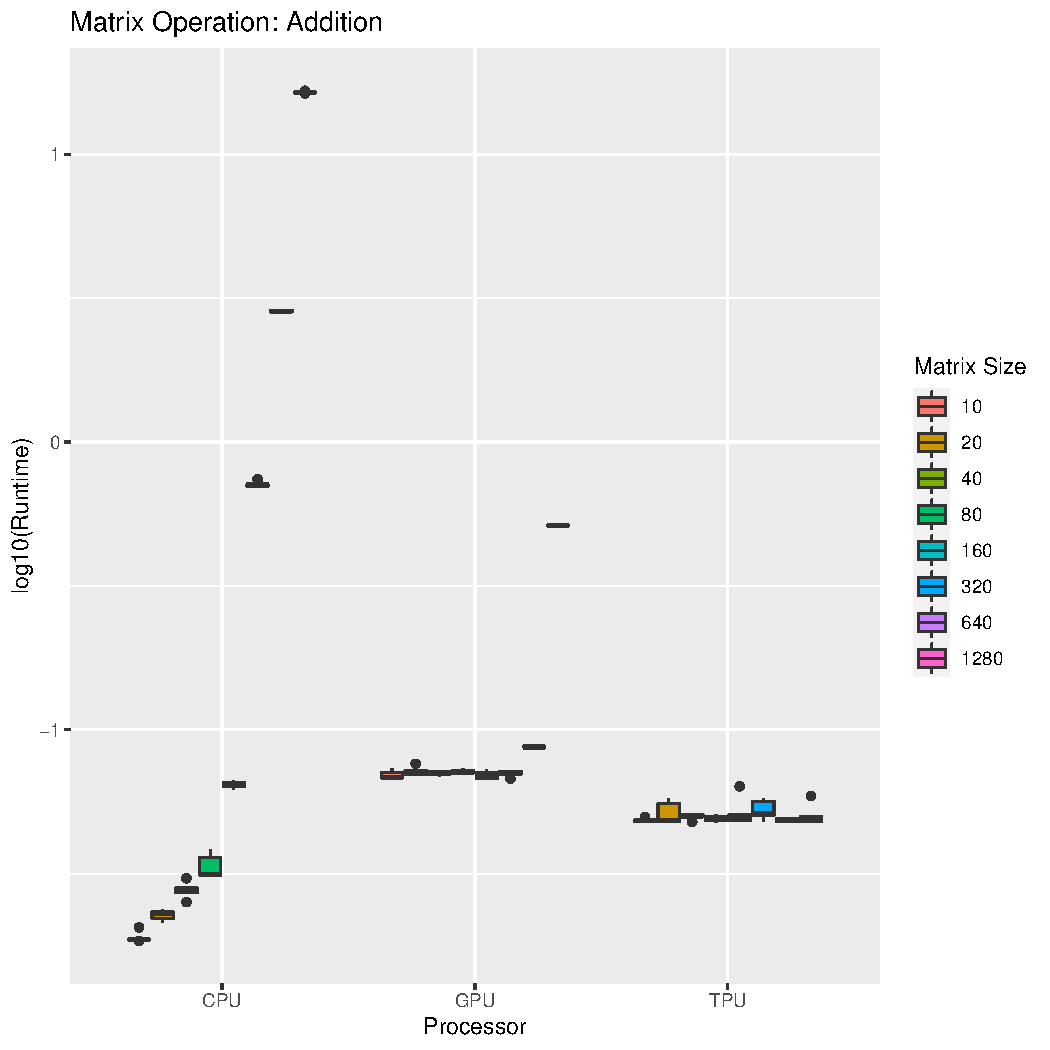
\includegraphics[page=1,width=0.5\linewidth]{../figs/operations_plots.pdf}
\includegraphics[page=2,width=0.5\linewidth]{../figs/operations_plots.pdf}
\includegraphics[page=3,width=0.5\linewidth]{../figs/operations_plots.pdf}
\caption{\label{fig:operation} Operation v.s. Processors for Each Matrix Size}
\end{figure}

\begin{figure}
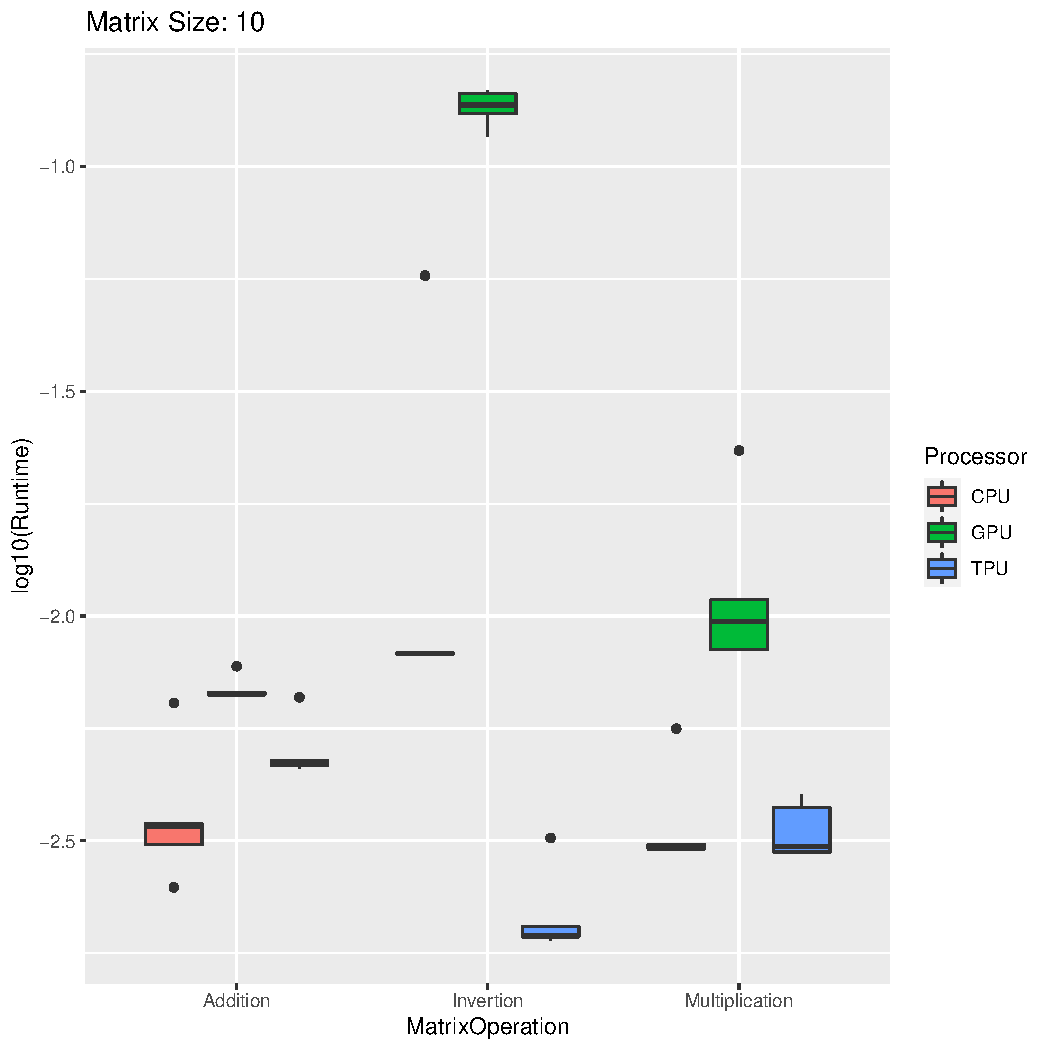
\includegraphics[page=1,width=0.333\linewidth]{../figs/size_plots.pdf}
\includegraphics[page=2,width=0.333\linewidth]{../figs/size_plots.pdf}
\includegraphics[page=3,width=0.333\linewidth]{../figs/size_plots.pdf}
\includegraphics[page=4,width=0.333\linewidth]{../figs/size_plots.pdf}
\includegraphics[page=5,width=0.333\linewidth]{../figs/size_plots.pdf}
\includegraphics[page=6,width=0.333\linewidth]{../figs/size_plots.pdf}
\includegraphics[page=7,width=0.333\linewidth]{../figs/size_plots.pdf}
\includegraphics[page=8,width=0.333\linewidth]{../figs/size_plots.pdf}
\includegraphics[page=9,width=0.333\linewidth]{../figs/size_plots.pdf}
\caption{\label{fig:Size} Matrix Size v.s. Operations for Each Processor.}
\end{figure}

\begin{figure}
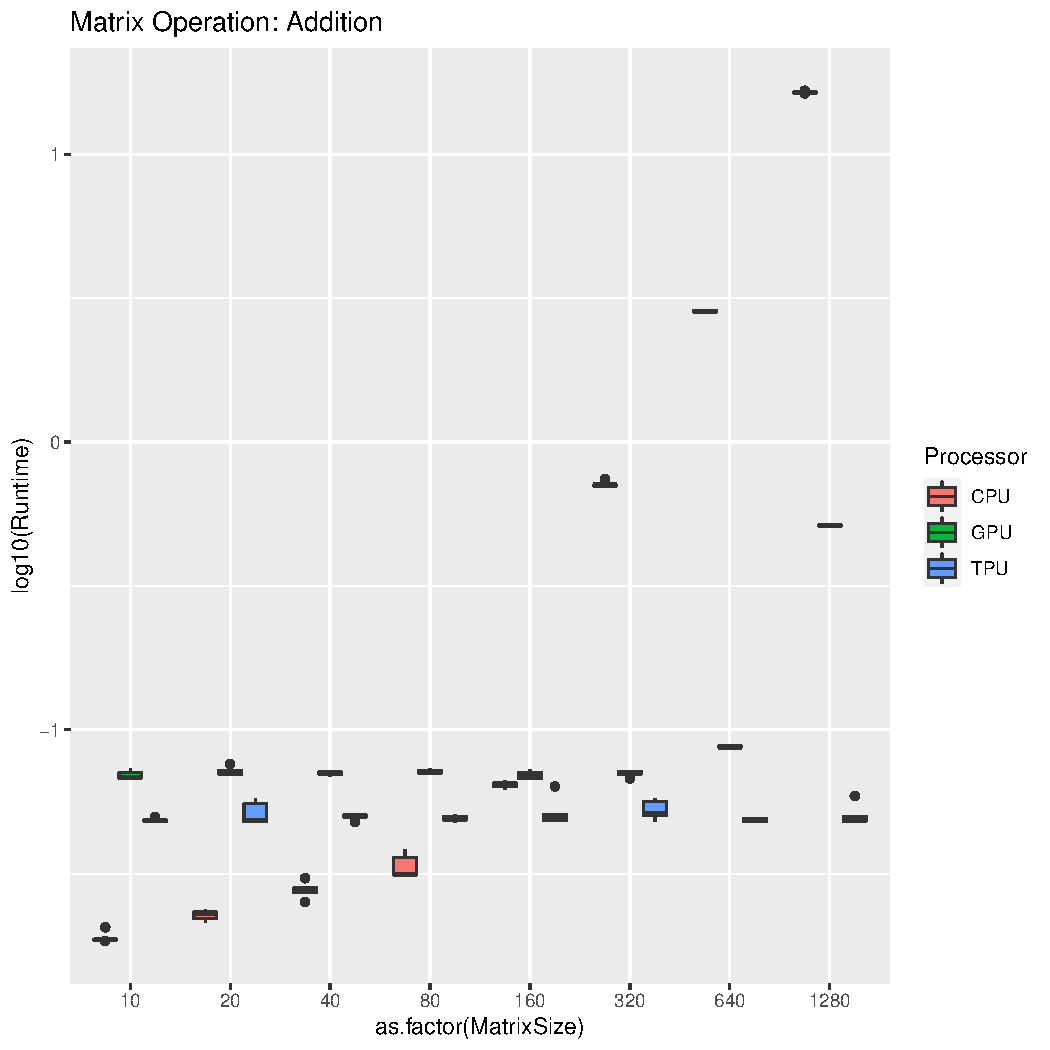
\includegraphics[page=1,width=0.5\linewidth]{../figs/operation_size.pdf}
\includegraphics[page=2,width=0.5\linewidth]{../figs/operation_size.pdf}
\includegraphics[page=3,width=0.5\linewidth]{../figs/operation_size.pdf}
\caption{\label{fig:operation_size} Operation v.s. Matrix Size for Each Processor}
\end{figure}

\hypertarget{lixian-chen-part-ii-plots}{%
\section{Lixian Chen Part II: Plots}\label{lixian-chen-part-ii-plots}}

\hypertarget{interaction-plots}{%
\subsection{Interaction Plots}\label{interaction-plots}}

\begin{Shaded}
\begin{Highlighting}[]
\KeywordTok{jpeg}\NormalTok{(}\DataTypeTok{filename =} \StringTok{"../figs/interaction\_size\_time.jpeg"}\NormalTok{, }\DataTypeTok{width =} \DecValTok{600}\NormalTok{, }\DataTypeTok{height =} \DecValTok{400}\NormalTok{,}\DataTypeTok{quality =} \DecValTok{10000}\NormalTok{)}
\KeywordTok{interaction.plot}\NormalTok{(df}\OperatorTok{$}\NormalTok{MatrixSize, df}\OperatorTok{$}\NormalTok{MatrixOperation, df}\OperatorTok{$}\NormalTok{Runtime)}
\ControlFlowTok{while}\NormalTok{ (}\OperatorTok{!}\KeywordTok{is.null}\NormalTok{(}\KeywordTok{dev.list}\NormalTok{()))  }\KeywordTok{dev.off}\NormalTok{()}
\end{Highlighting}
\end{Shaded}

\begin{center}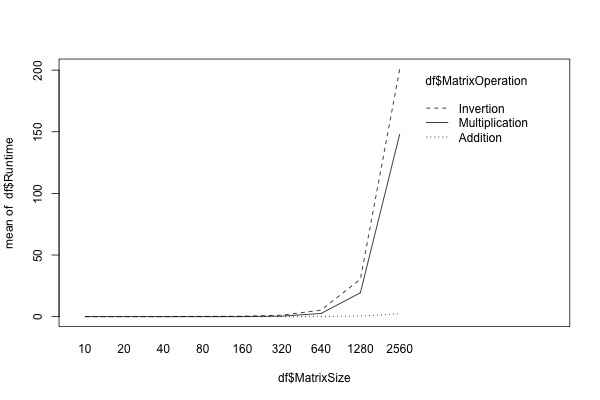
\includegraphics[width=0.9\linewidth]{../figs/interaction_size_time} \end{center}

\begin{Shaded}
\begin{Highlighting}[]
\KeywordTok{jpeg}\NormalTok{(}\DataTypeTok{filename =} \StringTok{"../figs/interaction\_size\_log\_time.jpeg"}\NormalTok{, }\DataTypeTok{width =} \DecValTok{600}\NormalTok{, }\DataTypeTok{height =} \DecValTok{400}\NormalTok{,}\DataTypeTok{quality =} \DecValTok{10000}\NormalTok{)}
\KeywordTok{interaction.plot}\NormalTok{(df}\OperatorTok{$}\NormalTok{MatrixSize, df}\OperatorTok{$}\NormalTok{MatrixOperation, }\KeywordTok{log}\NormalTok{(df}\OperatorTok{$}\NormalTok{Runtime))}
\ControlFlowTok{while}\NormalTok{ (}\OperatorTok{!}\KeywordTok{is.null}\NormalTok{(}\KeywordTok{dev.list}\NormalTok{()))  }\KeywordTok{dev.off}\NormalTok{()}
\end{Highlighting}
\end{Shaded}

\begin{center}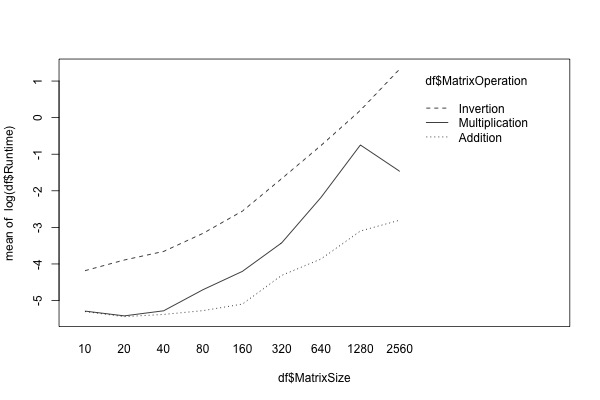
\includegraphics[width=0.9\linewidth]{../figs/interaction_size_log_time} \end{center}

\begin{Shaded}
\begin{Highlighting}[]
\KeywordTok{jpeg}\NormalTok{(}\DataTypeTok{filename =} \StringTok{"../figs/interaction\_CPU\_size\_time.jpeg"}\NormalTok{, }\DataTypeTok{width =} \DecValTok{600}\NormalTok{, }\DataTypeTok{height =} \DecValTok{400}\NormalTok{,}\DataTypeTok{quality =} \DecValTok{10000}\NormalTok{)}
\KeywordTok{interaction.plot}\NormalTok{(CPUdata}\OperatorTok{$}\NormalTok{MatrixSize, CPUdata}\OperatorTok{$}\NormalTok{MatrixOperation, CPUdata}\OperatorTok{$}\NormalTok{Runtime)}
\end{Highlighting}
\end{Shaded}

\begin{center}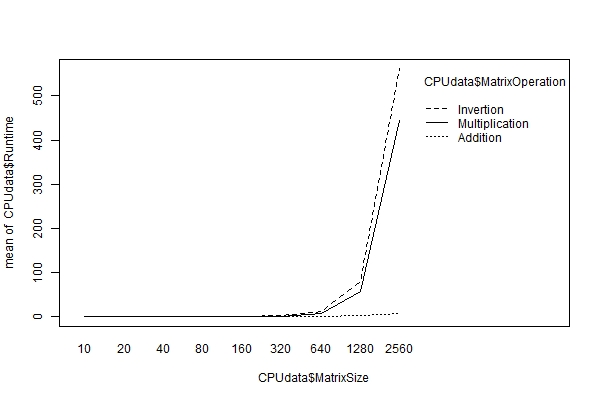
\includegraphics[width=0.9\linewidth]{../figs/interaction_CPU_size_time} \end{center}

\begin{Shaded}
\begin{Highlighting}[]
\KeywordTok{jpeg}\NormalTok{(}\DataTypeTok{filename =} \StringTok{"../figs/interaction\_GPU\_size\_time.jpeg"}\NormalTok{, }\DataTypeTok{width =} \DecValTok{600}\NormalTok{, }\DataTypeTok{height =} \DecValTok{400}\NormalTok{,}\DataTypeTok{quality =} \DecValTok{10000}\NormalTok{)}
\KeywordTok{interaction.plot}\NormalTok{(GPUdata}\OperatorTok{$}\NormalTok{MatrixSize, GPUdata}\OperatorTok{$}\NormalTok{MatrixOperation, GPUdata}\OperatorTok{$}\NormalTok{Runtime)}
\end{Highlighting}
\end{Shaded}

\begin{center}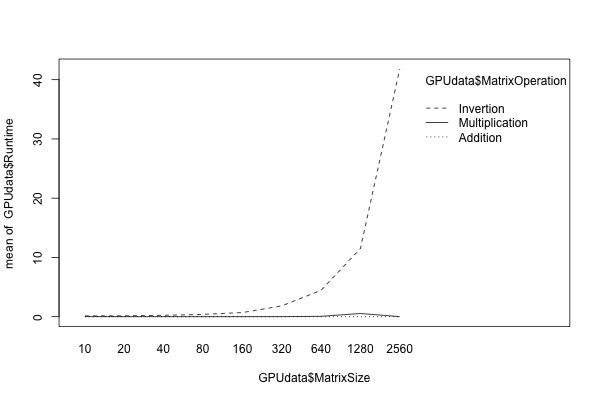
\includegraphics[width=0.9\linewidth]{../figs/interaction_GPU_size_time} \end{center}

\begin{Shaded}
\begin{Highlighting}[]
\KeywordTok{jpeg}\NormalTok{(}\DataTypeTok{filename =} \StringTok{"../figs/interaction\_TPU\_size\_time.jpeg"}\NormalTok{, }\DataTypeTok{width =} \DecValTok{600}\NormalTok{, }\DataTypeTok{height =} \DecValTok{400}\NormalTok{,}\DataTypeTok{quality =} \DecValTok{10000}\NormalTok{)}
\KeywordTok{interaction.plot}\NormalTok{(TPUdata}\OperatorTok{$}\NormalTok{MatrixSize, TPUdata}\OperatorTok{$}\NormalTok{MatrixOperation, TPUdata}\OperatorTok{$}\NormalTok{Runtime)}
\end{Highlighting}
\end{Shaded}

\begin{center}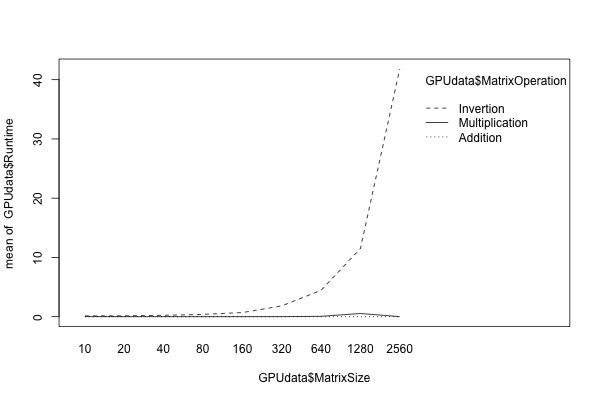
\includegraphics[width=0.9\linewidth]{../figs/interaction_GPU_size_time} \end{center}

\hypertarget{boxplots}{%
\subsection{Boxplots}\label{boxplots}}

\begin{Shaded}
\begin{Highlighting}[]
\KeywordTok{jpeg}\NormalTok{(}\DataTypeTok{filename =} \StringTok{"../figs/Operation\_vs\_runtime\_size320.jpeg"}\NormalTok{, }\DataTypeTok{width =} \DecValTok{700}\NormalTok{, }\DataTypeTok{height =} \DecValTok{400}\NormalTok{,}\DataTypeTok{quality =} \DecValTok{10000}\NormalTok{)}
\KeywordTok{boxplot}\NormalTok{(Runtime}\OperatorTok{\textasciitilde{}}\NormalTok{Processor}\OperatorTok{*}\NormalTok{MatrixOperation, }\DataTypeTok{data =}\NormalTok{ size320data, }\DataTypeTok{main=}\StringTok{"At the level of matrix size=320"}\NormalTok{)}
\end{Highlighting}
\end{Shaded}

\begin{center}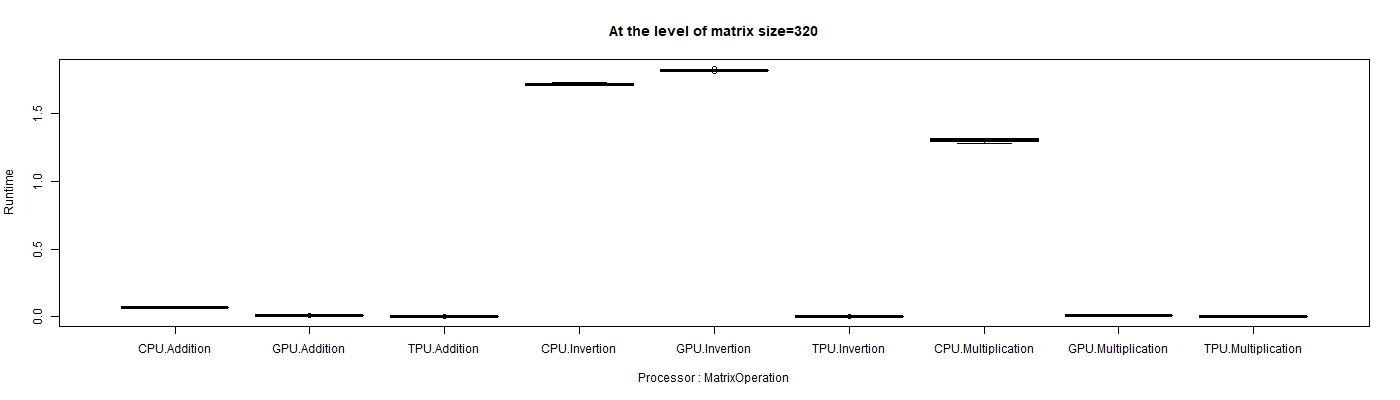
\includegraphics[width=0.9\linewidth]{../figs/Operation_vs_runtime_size320} \end{center}

\begin{Shaded}
\begin{Highlighting}[]
\KeywordTok{jpeg}\NormalTok{(}\DataTypeTok{filename =} \StringTok{"../figs/Operation\_vs\_runtime\_size640.jpeg"}\NormalTok{, }\DataTypeTok{width =} \DecValTok{700}\NormalTok{, }\DataTypeTok{height =} \DecValTok{400}\NormalTok{,}\DataTypeTok{quality =} \DecValTok{10000}\NormalTok{)}
\KeywordTok{boxplot}\NormalTok{(Runtime}\OperatorTok{\textasciitilde{}}\NormalTok{Processor}\OperatorTok{*}\NormalTok{MatrixOperation, }\DataTypeTok{data =}\NormalTok{ size640data, }\DataTypeTok{main=}\StringTok{"At the level of matrix size=640"}\NormalTok{)}
\end{Highlighting}
\end{Shaded}

\begin{center}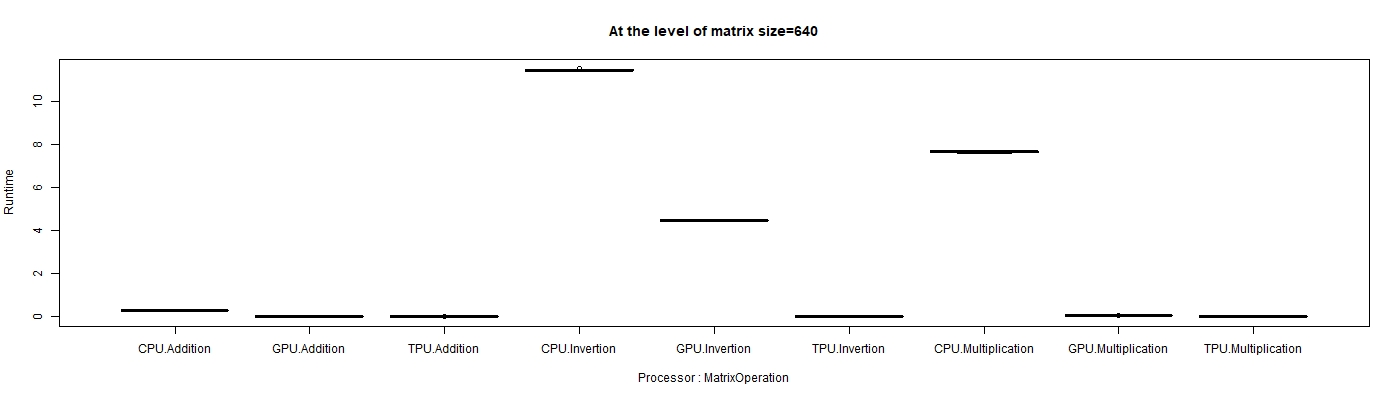
\includegraphics[width=0.9\linewidth]{../figs/Operation_vs_runtime_size640} \end{center}

\begin{Shaded}
\begin{Highlighting}[]
\KeywordTok{jpeg}\NormalTok{(}\DataTypeTok{filename =} \StringTok{"../figs/Operation\_vs\_runtime\_size1280.jpeg"}\NormalTok{, }\DataTypeTok{width =} \DecValTok{700}\NormalTok{, }\DataTypeTok{height =} \DecValTok{400}\NormalTok{,}\DataTypeTok{quality =} \DecValTok{10000}\NormalTok{)}
\KeywordTok{boxplot}\NormalTok{(Runtime}\OperatorTok{\textasciitilde{}}\NormalTok{Processor}\OperatorTok{*}\NormalTok{MatrixOperation, }\DataTypeTok{data =}\NormalTok{ size1280data, }\DataTypeTok{main=}\StringTok{"At the level of matrix size=1280"}\NormalTok{)}
\end{Highlighting}
\end{Shaded}

\begin{center}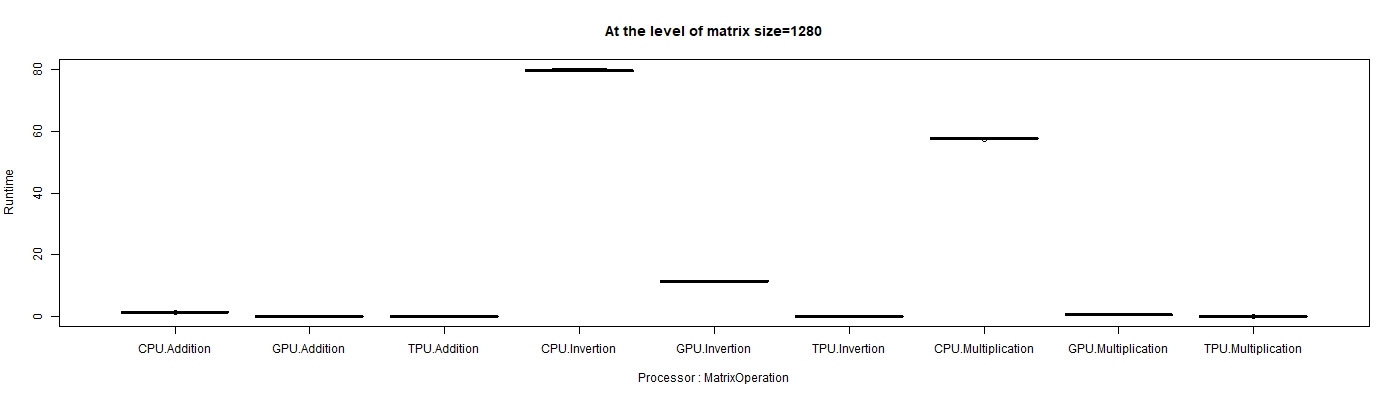
\includegraphics[width=0.9\linewidth]{../figs/Operation_vs_runtime_size1280} \end{center}

\begin{Shaded}
\begin{Highlighting}[]
\KeywordTok{jpeg}\NormalTok{(}\DataTypeTok{filename =} \StringTok{"../figs/Operation\_vs\_runtime\_size2560.jpeg"}\NormalTok{, }\DataTypeTok{width =} \DecValTok{700}\NormalTok{, }\DataTypeTok{height =} \DecValTok{400}\NormalTok{,}\DataTypeTok{quality =} \DecValTok{10000}\NormalTok{)}
\KeywordTok{boxplot}\NormalTok{(Runtime}\OperatorTok{\textasciitilde{}}\NormalTok{Processor}\OperatorTok{*}\NormalTok{MatrixOperation, }\DataTypeTok{data =}\NormalTok{ size2560data, }\DataTypeTok{main=}\StringTok{"At the level of matrix size=2560"}\NormalTok{)}
\end{Highlighting}
\end{Shaded}

\begin{center}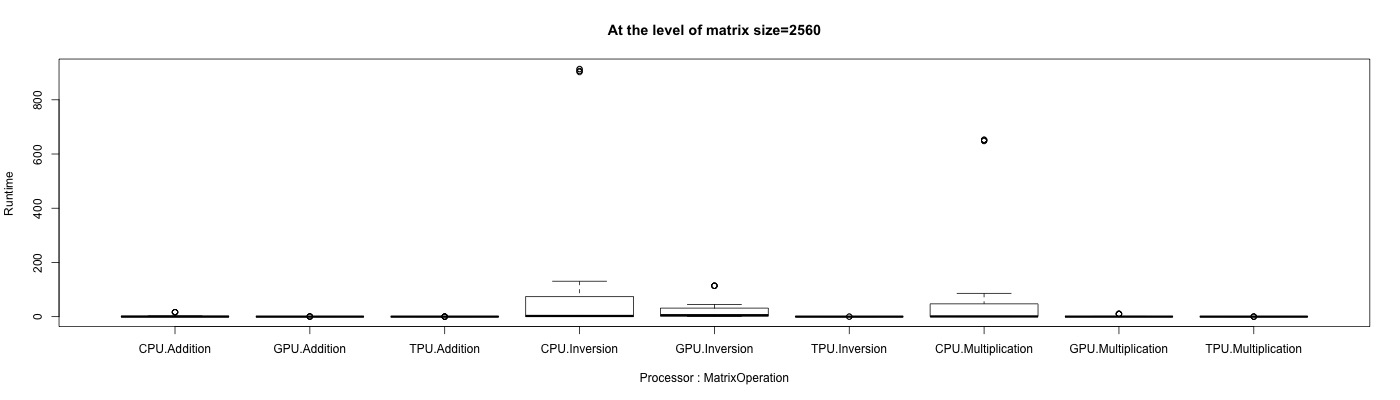
\includegraphics[width=0.9\linewidth]{../figs/Operation_vs_runtime_size2560} \end{center}

At the level of matrix size=2560, avoid using CPU for inversion and
multiplication because its run-times are much bigger.

\begin{Shaded}
\begin{Highlighting}[]
\CommentTok{\# Addition \& CPU}
\NormalTok{data[data}\OperatorTok{$}\NormalTok{Processor }\OperatorTok{==}\StringTok{ "CPU"} \OperatorTok{\&}\StringTok{ }\NormalTok{data}\OperatorTok{$}\NormalTok{MatrixOperation}\OperatorTok{==}\StringTok{"Addition"}\NormalTok{,] }\OperatorTok{\%\textgreater{}\%}
\KeywordTok{ggplot}\NormalTok{() }\OperatorTok{+}
\KeywordTok{geom\_point}\NormalTok{(}\DataTypeTok{mapping =} \KeywordTok{aes}\NormalTok{(}\DataTypeTok{x =}\NormalTok{ MatrixSize, }\DataTypeTok{y =} \KeywordTok{log}\NormalTok{(Runtime))) }\OperatorTok{+}
\KeywordTok{geom\_smooth}\NormalTok{(}\DataTypeTok{mapping =} \KeywordTok{aes}\NormalTok{(}\DataTypeTok{x =}\NormalTok{ MatrixSize, }\DataTypeTok{y =} \KeywordTok{log}\NormalTok{(Runtime))) }\OperatorTok{+}
\KeywordTok{labs}\NormalTok{(}\DataTypeTok{title =} \StringTok{"For CPU and Addition with Different Matrix Size"}\NormalTok{, }\DataTypeTok{x =} \StringTok{"Matrix Size"}\NormalTok{, }\DataTypeTok{y =} \StringTok{"Runtime"}\NormalTok{)}
\end{Highlighting}
\end{Shaded}

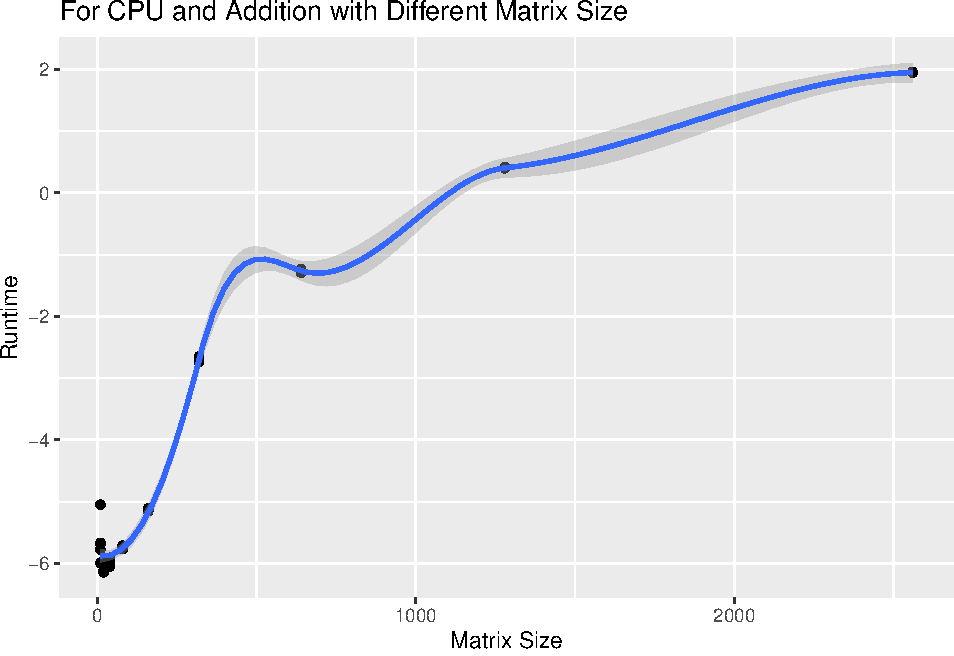
\includegraphics{main_files/figure-latex/unnamed-chunk-28-1.pdf}

\begin{Shaded}
\begin{Highlighting}[]
\CommentTok{\# Multiplication \& CPU}
\NormalTok{data[data}\OperatorTok{$}\NormalTok{Processor }\OperatorTok{==}\StringTok{ "CPU"} \OperatorTok{\&}\StringTok{ }\NormalTok{data}\OperatorTok{$}\NormalTok{MatrixOperation}\OperatorTok{==}\StringTok{"Multiplication"}\NormalTok{,] }\OperatorTok{\%\textgreater{}\%}
\KeywordTok{ggplot}\NormalTok{() }\OperatorTok{+}
\KeywordTok{geom\_point}\NormalTok{(}\DataTypeTok{mapping =} \KeywordTok{aes}\NormalTok{(}\DataTypeTok{x =}\NormalTok{ MatrixSize, }\DataTypeTok{y =} \KeywordTok{log}\NormalTok{(Runtime))) }\OperatorTok{+}
\KeywordTok{geom\_smooth}\NormalTok{(}\DataTypeTok{mapping =} \KeywordTok{aes}\NormalTok{(}\DataTypeTok{x =}\NormalTok{ MatrixSize, }\DataTypeTok{y =} \KeywordTok{log}\NormalTok{(Runtime))) }\OperatorTok{+}
\KeywordTok{labs}\NormalTok{(}\DataTypeTok{title =} \StringTok{"For CPU and Multiplication with Different Matrix Size"}\NormalTok{, }\DataTypeTok{x =} \StringTok{"Matrix Size"}\NormalTok{, }\DataTypeTok{y =} \StringTok{"Runtime"}\NormalTok{)}
\end{Highlighting}
\end{Shaded}

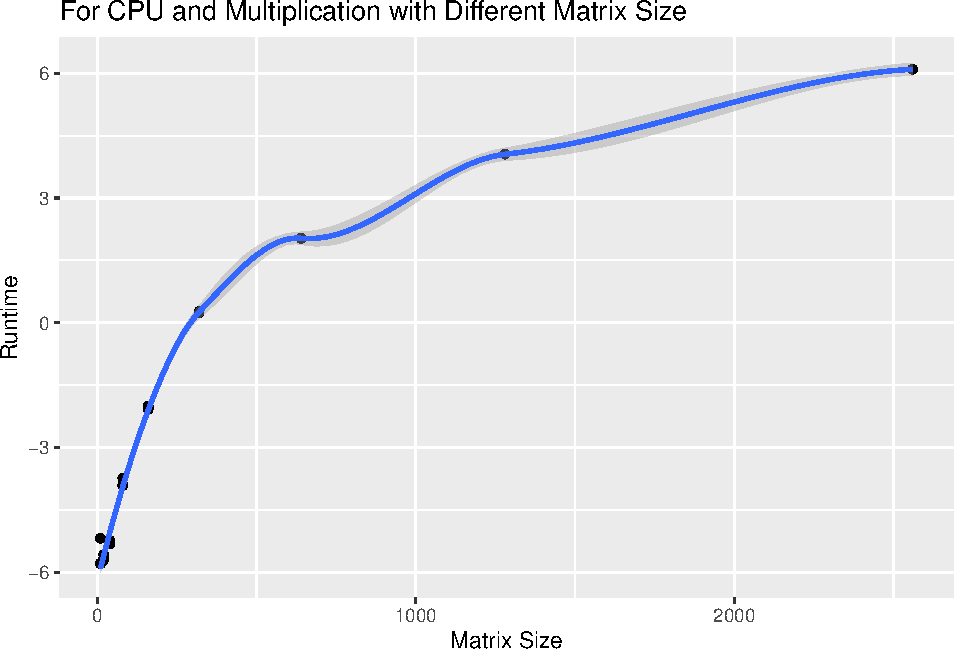
\includegraphics{main_files/figure-latex/unnamed-chunk-28-2.pdf}

\begin{Shaded}
\begin{Highlighting}[]
\CommentTok{\# Invertion \& CPU}
\NormalTok{data[data}\OperatorTok{$}\NormalTok{Processor }\OperatorTok{==}\StringTok{ "CPU"} \OperatorTok{\&}\StringTok{ }\NormalTok{data}\OperatorTok{$}\NormalTok{MatrixOperation}\OperatorTok{==}\StringTok{"Invertion"}\NormalTok{,] }\OperatorTok{\%\textgreater{}\%}
\KeywordTok{ggplot}\NormalTok{() }\OperatorTok{+}
\KeywordTok{geom\_point}\NormalTok{(}\DataTypeTok{mapping =} \KeywordTok{aes}\NormalTok{(}\DataTypeTok{x =}\NormalTok{ MatrixSize, }\DataTypeTok{y =} \KeywordTok{log}\NormalTok{(Runtime))) }\OperatorTok{+}
\KeywordTok{geom\_smooth}\NormalTok{(}\DataTypeTok{mapping =} \KeywordTok{aes}\NormalTok{(}\DataTypeTok{x =}\NormalTok{ MatrixSize, }\DataTypeTok{y =} \KeywordTok{log}\NormalTok{(Runtime))) }\OperatorTok{+}
\KeywordTok{labs}\NormalTok{(}\DataTypeTok{title =} \StringTok{"For CPU and Invertion with Different Matrix Size"}\NormalTok{, }\DataTypeTok{x =} \StringTok{"Matrix Size"}\NormalTok{, }\DataTypeTok{y =} \StringTok{"Runtime"}\NormalTok{)}
\end{Highlighting}
\end{Shaded}

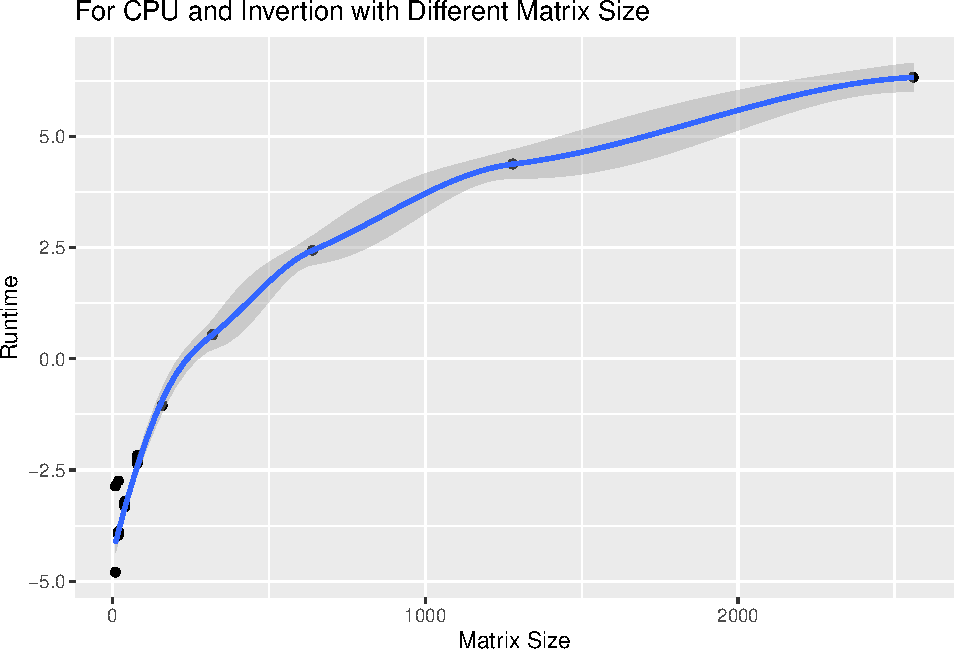
\includegraphics{main_files/figure-latex/unnamed-chunk-28-3.pdf}

\begin{Shaded}
\begin{Highlighting}[]
\CommentTok{\# Addition \& GPU}
\NormalTok{data[data}\OperatorTok{$}\NormalTok{Processor }\OperatorTok{==}\StringTok{ "GPU"} \OperatorTok{\&}\StringTok{ }\NormalTok{data}\OperatorTok{$}\NormalTok{MatrixOperation}\OperatorTok{==}\StringTok{"Addition"}\NormalTok{,] }\OperatorTok{\%\textgreater{}\%}
\KeywordTok{ggplot}\NormalTok{() }\OperatorTok{+}
\KeywordTok{geom\_point}\NormalTok{(}\DataTypeTok{mapping =} \KeywordTok{aes}\NormalTok{(}\DataTypeTok{x =}\NormalTok{ MatrixSize, }\DataTypeTok{y =} \KeywordTok{log}\NormalTok{(Runtime))) }\OperatorTok{+}
\KeywordTok{geom\_smooth}\NormalTok{(}\DataTypeTok{mapping =} \KeywordTok{aes}\NormalTok{(}\DataTypeTok{x =}\NormalTok{ MatrixSize, }\DataTypeTok{y =} \KeywordTok{log}\NormalTok{(Runtime))) }\OperatorTok{+}
\KeywordTok{labs}\NormalTok{(}\DataTypeTok{title =} \StringTok{"For GPU and Addition with Different Matrix Size"}\NormalTok{, }\DataTypeTok{x =} \StringTok{"Matrix Size"}\NormalTok{, }\DataTypeTok{y =} \StringTok{"Runtime"}\NormalTok{)}
\end{Highlighting}
\end{Shaded}

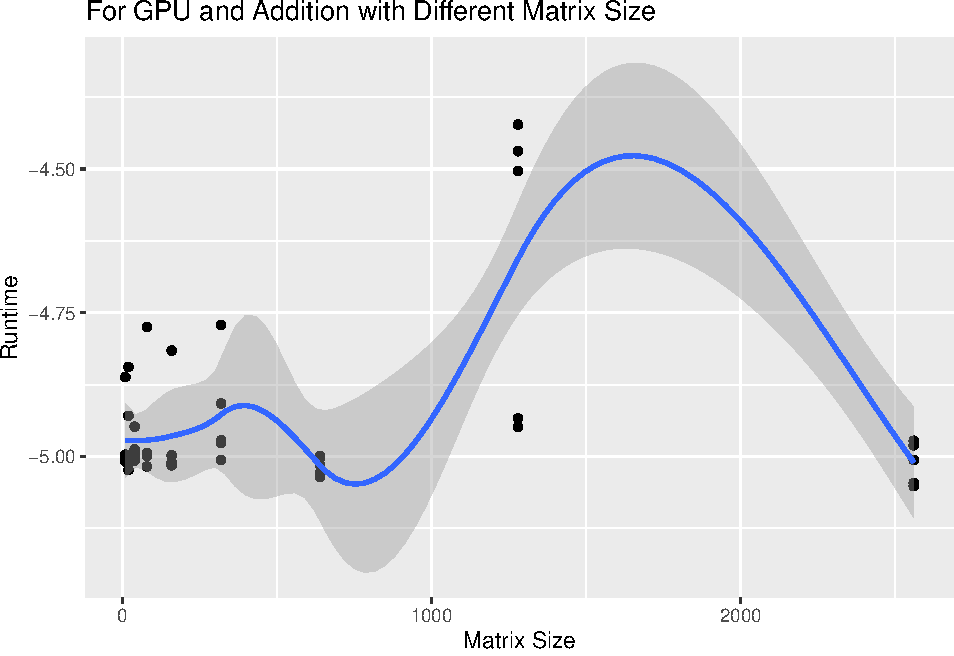
\includegraphics{main_files/figure-latex/unnamed-chunk-28-4.pdf}

\begin{Shaded}
\begin{Highlighting}[]
\CommentTok{\# Multiplication \& GPU}
\NormalTok{data[data}\OperatorTok{$}\NormalTok{Processor }\OperatorTok{==}\StringTok{ "GPU"} \OperatorTok{\&}\StringTok{ }\NormalTok{data}\OperatorTok{$}\NormalTok{MatrixOperation}\OperatorTok{==}\StringTok{"Multiplication"}\NormalTok{,] }\OperatorTok{\%\textgreater{}\%}
\KeywordTok{ggplot}\NormalTok{() }\OperatorTok{+}
\KeywordTok{geom\_point}\NormalTok{(}\DataTypeTok{mapping =} \KeywordTok{aes}\NormalTok{(}\DataTypeTok{x =}\NormalTok{ MatrixSize, }\DataTypeTok{y =} \KeywordTok{log}\NormalTok{(Runtime))) }\OperatorTok{+}
\KeywordTok{geom\_smooth}\NormalTok{(}\DataTypeTok{mapping =} \KeywordTok{aes}\NormalTok{(}\DataTypeTok{x =}\NormalTok{ MatrixSize, }\DataTypeTok{y =} \KeywordTok{log}\NormalTok{(Runtime))) }\OperatorTok{+}
\KeywordTok{labs}\NormalTok{(}\DataTypeTok{title =} \StringTok{"For CPU and Multiplication with Different Matrix Size"}\NormalTok{, }\DataTypeTok{x =} \StringTok{"Matrix Size"}\NormalTok{, }\DataTypeTok{y =} \StringTok{"Runtime"}\NormalTok{)}
\end{Highlighting}
\end{Shaded}

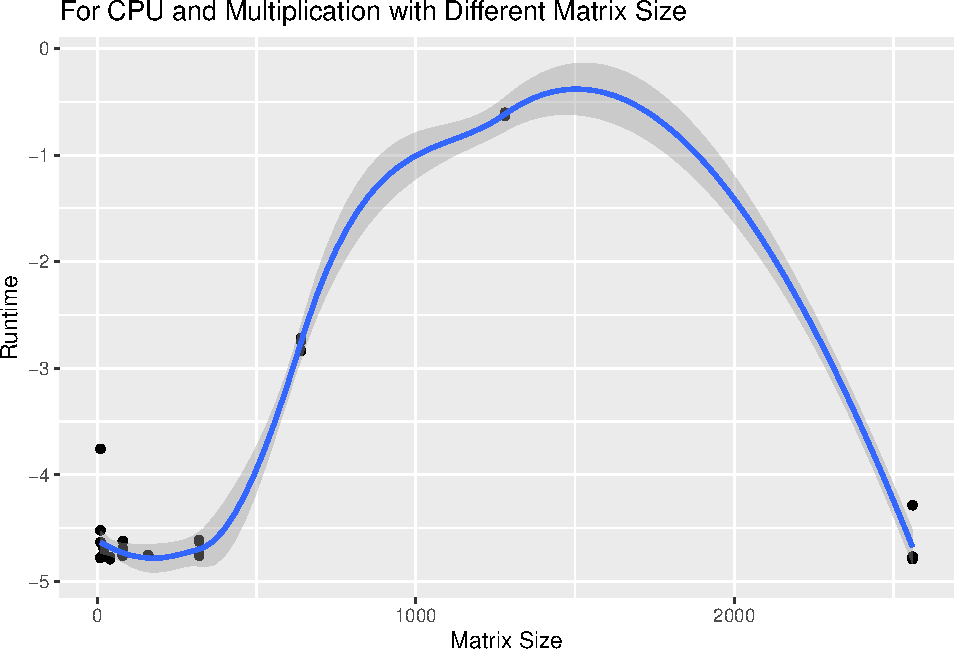
\includegraphics{main_files/figure-latex/unnamed-chunk-28-5.pdf}

\begin{Shaded}
\begin{Highlighting}[]
\CommentTok{\# Invertion \& GPU}
\NormalTok{data[data}\OperatorTok{$}\NormalTok{Processor }\OperatorTok{==}\StringTok{ "GPU"} \OperatorTok{\&}\StringTok{ }\NormalTok{data}\OperatorTok{$}\NormalTok{MatrixOperation}\OperatorTok{==}\StringTok{"Invertion"}\NormalTok{,] }\OperatorTok{\%\textgreater{}\%}
\KeywordTok{ggplot}\NormalTok{() }\OperatorTok{+}
\KeywordTok{geom\_point}\NormalTok{(}\DataTypeTok{mapping =} \KeywordTok{aes}\NormalTok{(}\DataTypeTok{x =}\NormalTok{ MatrixSize, }\DataTypeTok{y =} \KeywordTok{log}\NormalTok{(Runtime))) }\OperatorTok{+}
\KeywordTok{geom\_smooth}\NormalTok{(}\DataTypeTok{mapping =} \KeywordTok{aes}\NormalTok{(}\DataTypeTok{x =}\NormalTok{ MatrixSize, }\DataTypeTok{y =} \KeywordTok{log}\NormalTok{(Runtime))) }\OperatorTok{+}
\KeywordTok{labs}\NormalTok{(}\DataTypeTok{title =} \StringTok{"For CPU and Invertion with Different Matrix Size"}\NormalTok{, }\DataTypeTok{x =} \StringTok{"Matrix Size"}\NormalTok{, }\DataTypeTok{y =} \StringTok{"Runtime"}\NormalTok{)}
\end{Highlighting}
\end{Shaded}

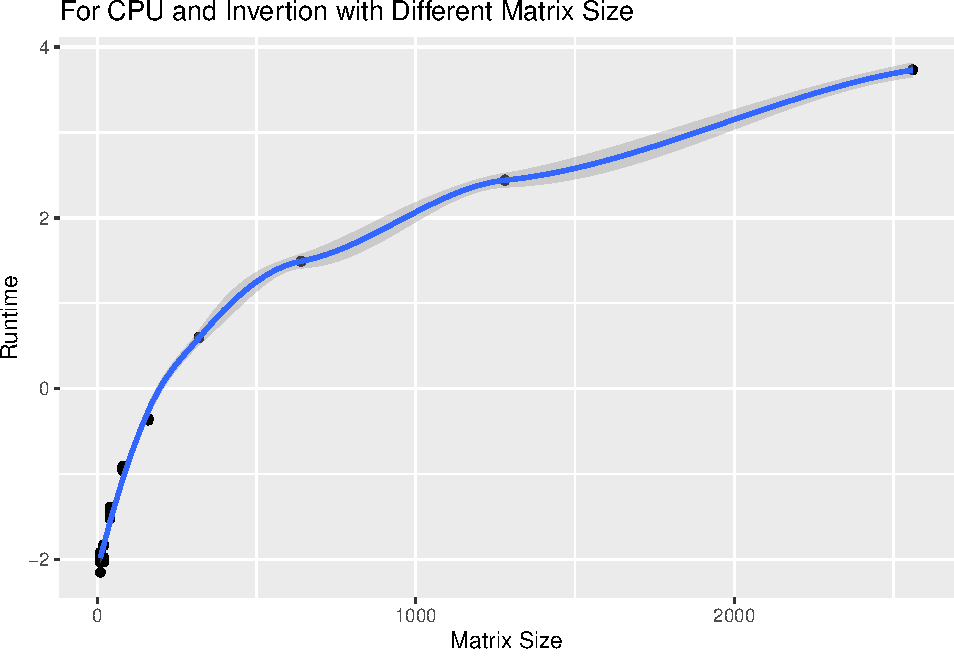
\includegraphics{main_files/figure-latex/unnamed-chunk-28-6.pdf}

\begin{Shaded}
\begin{Highlighting}[]
\CommentTok{\# Addition \& TPU}
\NormalTok{data[data}\OperatorTok{$}\NormalTok{Processor }\OperatorTok{==}\StringTok{ "TPU"} \OperatorTok{\&}\StringTok{ }\NormalTok{data}\OperatorTok{$}\NormalTok{MatrixOperation}\OperatorTok{==}\StringTok{"Addition"}\NormalTok{,] }\OperatorTok{\%\textgreater{}\%}
\KeywordTok{ggplot}\NormalTok{() }\OperatorTok{+}
\KeywordTok{geom\_point}\NormalTok{(}\DataTypeTok{mapping =} \KeywordTok{aes}\NormalTok{(}\DataTypeTok{x =}\NormalTok{ MatrixSize, }\DataTypeTok{y =} \KeywordTok{log}\NormalTok{(Runtime))) }\OperatorTok{+}
\KeywordTok{geom\_smooth}\NormalTok{(}\DataTypeTok{mapping =} \KeywordTok{aes}\NormalTok{(}\DataTypeTok{x =}\NormalTok{ MatrixSize, }\DataTypeTok{y =} \KeywordTok{log}\NormalTok{(Runtime))) }\OperatorTok{+}
\KeywordTok{labs}\NormalTok{(}\DataTypeTok{title =} \StringTok{"For TPU and Addition with Different Matrix Size"}\NormalTok{, }\DataTypeTok{x =} \StringTok{"Matrix Size"}\NormalTok{, }\DataTypeTok{y =} \StringTok{"Runtime"}\NormalTok{)}
\end{Highlighting}
\end{Shaded}

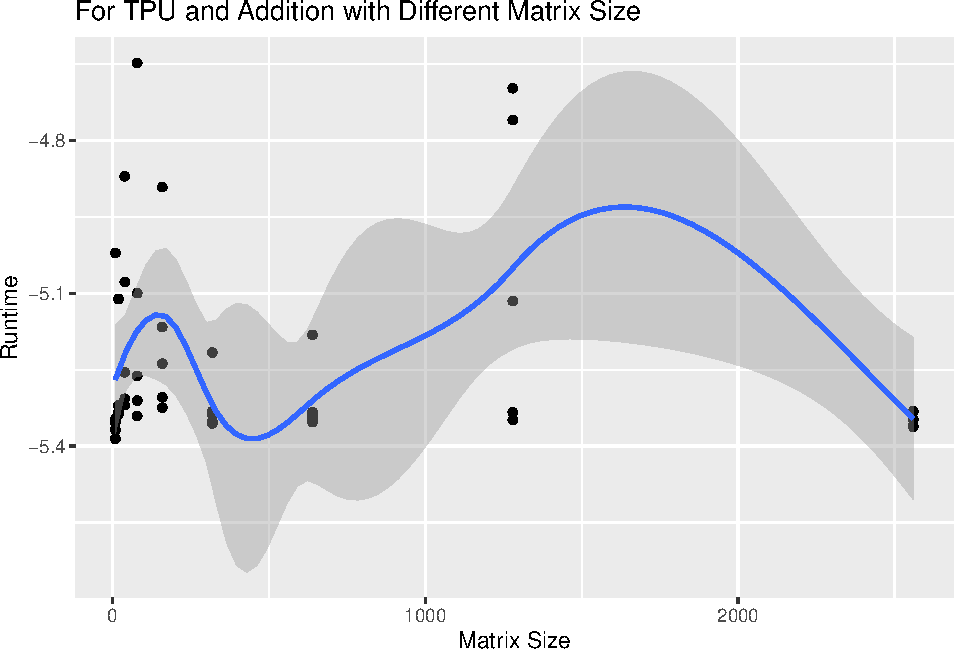
\includegraphics{main_files/figure-latex/unnamed-chunk-28-7.pdf}

\begin{Shaded}
\begin{Highlighting}[]
\CommentTok{\# Multiplication \& TPU}
\NormalTok{data[data}\OperatorTok{$}\NormalTok{Processor }\OperatorTok{==}\StringTok{ "TPU"} \OperatorTok{\&}\StringTok{ }\NormalTok{data}\OperatorTok{$}\NormalTok{MatrixOperation}\OperatorTok{==}\StringTok{"Multiplication"}\NormalTok{,] }\OperatorTok{\%\textgreater{}\%}
\KeywordTok{ggplot}\NormalTok{() }\OperatorTok{+}
\KeywordTok{geom\_point}\NormalTok{(}\DataTypeTok{mapping =} \KeywordTok{aes}\NormalTok{(}\DataTypeTok{x =}\NormalTok{ MatrixSize, }\DataTypeTok{y =} \KeywordTok{log}\NormalTok{(Runtime))) }\OperatorTok{+}
\KeywordTok{geom\_smooth}\NormalTok{(}\DataTypeTok{mapping =} \KeywordTok{aes}\NormalTok{(}\DataTypeTok{x =}\NormalTok{ MatrixSize, }\DataTypeTok{y =} \KeywordTok{log}\NormalTok{(Runtime))) }\OperatorTok{+}
\KeywordTok{labs}\NormalTok{(}\DataTypeTok{title =} \StringTok{"For TPU and Multiplication with Different Matrix Size"}\NormalTok{, }\DataTypeTok{x =} \StringTok{"Matrix Size"}\NormalTok{, }\DataTypeTok{y =} \StringTok{"Runtime"}\NormalTok{)}
\end{Highlighting}
\end{Shaded}

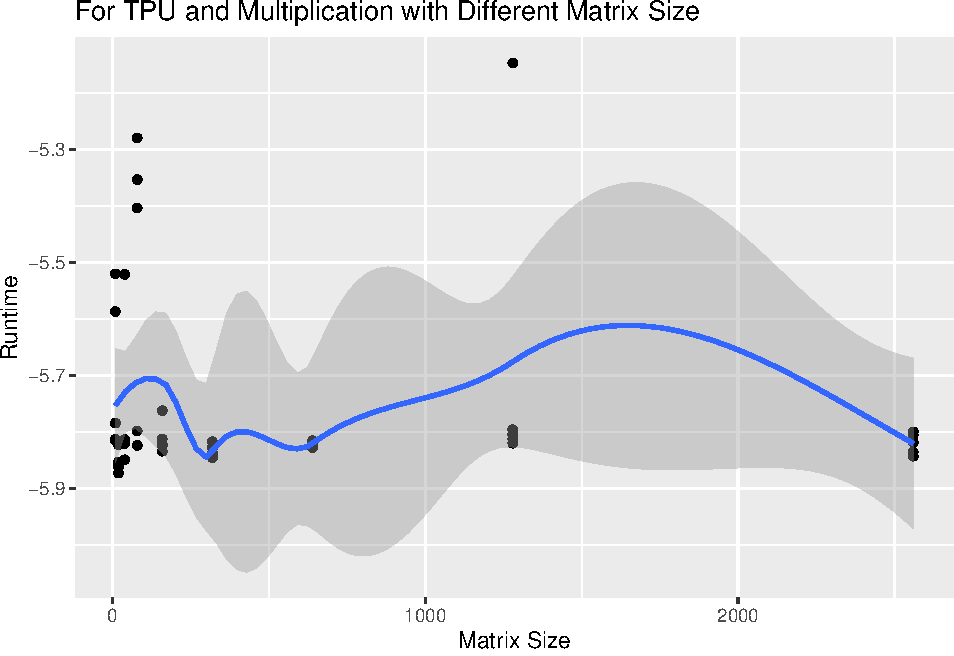
\includegraphics{main_files/figure-latex/unnamed-chunk-28-8.pdf}

\begin{Shaded}
\begin{Highlighting}[]
\CommentTok{\# Invertion \& TPU}
\NormalTok{data[data}\OperatorTok{$}\NormalTok{Processor }\OperatorTok{==}\StringTok{ "TPU"} \OperatorTok{\&}\StringTok{ }\NormalTok{data}\OperatorTok{$}\NormalTok{MatrixOperation}\OperatorTok{==}\StringTok{"Invertion"}\NormalTok{,] }\OperatorTok{\%\textgreater{}\%}
\KeywordTok{ggplot}\NormalTok{() }\OperatorTok{+}
\KeywordTok{geom\_point}\NormalTok{(}\DataTypeTok{mapping =} \KeywordTok{aes}\NormalTok{(}\DataTypeTok{x =}\NormalTok{ MatrixSize, }\DataTypeTok{y =} \KeywordTok{log}\NormalTok{(Runtime))) }\OperatorTok{+}
\KeywordTok{geom\_smooth}\NormalTok{(}\DataTypeTok{mapping =} \KeywordTok{aes}\NormalTok{(}\DataTypeTok{x =}\NormalTok{ MatrixSize, }\DataTypeTok{y =} \KeywordTok{log}\NormalTok{(Runtime))) }\OperatorTok{+}
\KeywordTok{labs}\NormalTok{(}\DataTypeTok{title =} \StringTok{"For TPU and Invertion with Different Matrix Size"}\NormalTok{, }\DataTypeTok{x =} \StringTok{"Matrix Size"}\NormalTok{, }\DataTypeTok{y =} \StringTok{"Runtime"}\NormalTok{)}
\end{Highlighting}
\end{Shaded}

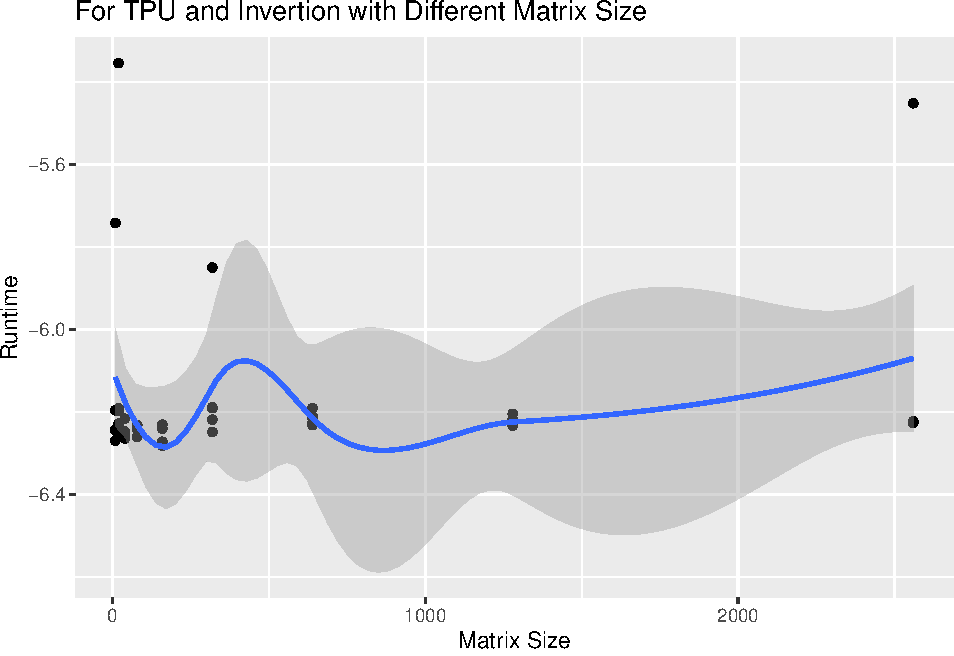
\includegraphics{main_files/figure-latex/unnamed-chunk-28-9.pdf}

\end{document}
